\documentclass[MSc, french]{ulthese} % https://gitlab.com/vigou3/ulthese/
\usepackage{chapterbib}
\usepackage{natbib}
\usepackage{amsmath}
\usepackage{icomma}
\usepackage{longtable}
\usepackage{tabularx}
\usepackage{booktabs}
\usepackage{graphicx}
\usepackage{float}
\usepackage{amssymb, amsmath, amsthm}
\usepackage{caption}
\usepackage{pgfplotstable}
\usepackage{pgffor}
\usepackage{subcaption}
\pgfplotsset{compat=1.18}
\usepackage{pgfplots}
\usepackage[T1]{fontenc}
\usepackage{lipsum}
\usepackage{tikz}
\usetikzlibrary{arrows.meta, positioning, shapes.geometric}

\usepackage[unicode, bookmarks=false]{hyperref}


\theoremstyle{definition}

\newtheorem{theorem}{Théorème}
\newtheorem{lemma}[theorem]{Lemme}
\newtheorem{corollary}[theorem]{Corollaire}
\newtheorem{proposition}[theorem]{Proposition}
\newtheorem{definition}{Définition}
\newtheorem{example}[theorem]{Exemple}
\newtheorem{remark}{Remarque}
\newtheorem{notation}[theorem]{Notation}


\titre{L'effet de l'arsenic aéroporté PM2.5 sur les maladies respiratoires chroniques : une analyse des données provenant des États-Unis}
\auteur{José Manuel Rodr\'iguez Caballero}
\programme{Maîtrise en Statistiques}
\direction{M'Hamed Lajmi Lakhal Chaieb}
\codirection{Karim Barigou}
\annee{2025}

\begin{document}

\frontmatter                    % pages liminaires

\frontispice                    % production de la page frontispice

%\include{resume}                % résumé français

%\include{abstract}              % résumé anglais

\cleardoublepage

\tableofcontents                % production de la TdM
\cleardoublepage

\listoftables                   % production de la liste des tableaux
\cleardoublepage

\listoffigures                  % production de la liste des figures
\cleardoublepage

%\include{remerciements}         % remerciements
%\include{avantpropos}           % avant-propos

\mainmatter                     % corps du document

%\include{introduction}
\chapter{\'Etat de l'Art}
\label{ch:stateart}

\section{Introduction et importance de la problématique}
La pollution de l’air est reconnue depuis plusieurs décennies comme un enjeu majeur de santé publique. Elle est associée à un large éventail d’effets néfastes sur la santé, dont une proportion importante de pathologies respiratoires chroniques (bronchites chroniques, asthme, cancer du poumon, etc.) \citep{Bang2015,Donaldson2010,Mazurek2017}. Les maladies respiratoires liées à l’exposition chronique ou aiguë à des polluants atmosphériques constituent en effet un défi épidémiologique et socio-économique, car elles mobilisent des ressources médicales importantes et engendrent des pertes de productivité.

Les études épidémiologiques mettent en évidence l’existence d’une corrélation robuste entre l’exposition à divers polluants de l’air (particules fines PM\textsubscript{2.5} et PM\textsubscript{10}, gaz, fibres, etc.) et la survenue ou l’aggravation de maladies respiratoires \citep{Cho2011,Gomes2014}. Au-delà de la corrélation, l’établissement d’un lien de causalité exige une modélisation statistique et mécanistique précise, prenant en compte la dynamique d’exposition, les mécanismes biologiques sous-jacents et la présence de facteurs confondants (âge, statut socio-économique, co-expositions, etc.).

Parmi les travaux de grande ampleur, le \emph{National Morbidity, Mortality, and Air Pollution Study (NMMAPS)} illustre l’importance des méthodes novatrices, de leur implémentation dans \textsf{R}, et des outils de recherche reproductible pour produire des résultats solides \citep{DominiciMcDermottDaniels2003,SametDominiciZeger2000,SametZegerDominici2000,SametDominiciCurriero2000,DominiciSametZeger2000,BellMcDermottZeger2004,PengDominiciPastorBarriuso2005,DominiciPengZeger2007}. Plus généralement, l’épidémiologie de la pollution atmosphérique recourt à quatre principaux types de plans d’étude :

\begin{enumerate}
	\item les \emph{études temporelles} (\emph{time series} dites ``écologiques"),
	\item les études de type \emph{case-crossover},
	\item les études de panel,
	\item les études de cohorte.
\end{enumerate}

Nous présentons ci-dessous ces designs, leurs modèles statistiques habituels, ainsi que quelques exemples d’applications.


\subsection{Études temporelles (\emph{time series studies})}
Les \emph{études temporelles} relient les expositions et les issues de santé au cours du temps en exploitant des données agrégées au plan quotidien (p.~ex. nombre de décès ou d’hospitalisations) et des niveaux de pollution journaliers mesurés par des stations fixes \citep{BellSametDominici2004}. Ces travaux s’appuient généralement sur des modèles de régression, de type \emph{Generalized Linear Models (GLM)} ou \emph{Generalized Additive Models (GAM)}, afin d’estimer l’effet de la pollution sur la mortalité ou la morbidité tout en prenant en compte les fluctuations lentes (saisonnalité, tendance à long terme) via l’utilisation de fonctions de lissage (p.~ex. splines cubiques ou loess) \citep{McCullaghNelder1989,HastieTibshirani1990}.

Le \emph{NMMAPS} constitue la plus vaste étude de ce type à ce jour \citep{DominiciMcDermottDaniels2003,SametDominiciZeger2000,SametZegerDominici2000,SametDominiciCurriero2000,DominiciPengZeger2007,BellMcDermottZeger2004,PengDominiciPastorBarriuso2005,DominiciSametZeger2000}. Contrairement à la plupart des études temporelles antérieures, souvent monocentriques, le \emph{NMMAPS} inclut des données de dizaines de villes américaines et fournit des estimations spécifiques à chaque localité, à l’échelle régionale et nationale, notamment pour les particules fines (PM\textsubscript{10}) et la mortalité. Des modèles hiérarchiques (``multiniveaux'') y consolident les estimations issues de différentes localités \citep{DominiciSametZeger2000}.

\subsection{Études de type \emph{case-crossover}}
La conception \emph{case-crossover} \citep{Maclure1991,Jaakkola2003,MaclureMittleman2000} a été développée pour étudier des effets aigus et transitoires d’expositions intermittentes \citep{BreslowDay1980,Schlesselman1994}. Chaque individu qui développe l’événement (le ``cas'') sert de son propre témoin (``contrôle''), ce qui permet de diminuer l’impact des variables de confusion invariantes dans le temps (âge, sexe, tabagisme, etc.). Dans les études de pollution atmosphérique, ce design se révèle particulièrement adapté lorsque l’exposition présente de fortes variations journalières et que l’issue de santé (par exemple, une crise d’asthme) est aiguë \citep{MaclureMittleman2000,Jaakkola2003}.

Deux biais majeurs ont été identifiés : 

\begin{enumerate}
	\item la présence de tendance à long terme et de saisonnalité dans les concentrations de polluants, qui viole l’hypothèse de stationnarité de la série temporelle \citep{Navidi1998,BatesonSchwartz1999,LumleyLevy2000,BatesonSchwartz2001,LevyLumleySheppard2001},
	\item l’``overlap bias'' (recouvrement des périodes de référence) \citep{AustinFlandersRothman1989,LumleyLevy2000,JanesSheppardLumley2005a,JanesSheppardLumley2005b}. 
\end{enumerate}

Malgré cela, plusieurs études monocentriques et multicentriques ont mis en œuvre cette approche \citep{SchwartzLee1999,NeasSchwartzDockery1999,PetersDockeryMuller2001,LevySheppardCheckoway2001,D'IppolitiForastiereAncona2003,SymonsWangGuallar2006,ZanobettiSchwartz2005,BarnettWilliamsSchwartz2005,BarnettWilliamsSchwartz2006,MedinaRamónZanobetti2006}.

Par exemple, Levy et al. \citep{LevySheppardCheckoway2001} n’ont pas observé d’effet significatif d’une hausse à court terme des particules PM sur le risque d’arrêt cardiaque soudain chez des sujets sans antécédent cardiovasculaire, tandis que Peters et al. \citep{PetersKlotzHeier2004} ont mis en évidence un lien entre la pollution liée au trafic et la survenue d’infarctus du myocarde chez des sujets à risque.

\subsection{Études de panel}
Les \emph{études de panel} consistent à suivre un même groupe d’individus pendant une période de temps, en mesurant régulièrement l’exposition et l’issue de santé \citep{PetersAvolGauderman1999,PetersAvolNavidi1999,GaudermanMcConnellGilliland2000}. Elles sont adaptées à l’étude d’effets aigus dans des sous-populations susceptibles (enfants, personnes âgées, patients atteints de BPCO, etc.). Les mesures de santé peuvent être répétées (p.~ex. plusieurs mesures de la fonction respiratoire) et l’exposition peut être évaluée via des capteurs individuels ou des stations fixes. L’un des exemples les plus connus est la \emph{Children’s Health Study} en Californie du Sud \citep{PetersAvolNavidi1999,PetersAvolGauderman1999,GaudermanMcConnellGilliland2000}, qui a utilisé des modèles mixtes (\emph{linear mixed models}) pour mettre en évidence un lien entre l’exposition chronique aux particules fines, au NO\textsubscript{2} et la réduction de la croissance pulmonaire chez l’enfant \citep{GaudermanMcConnellGilliland2000}.

\subsection{Études de cohorte}
Les \emph{études de cohorte} \citep{BellSametDominici2004} évaluent l’impact d’une exposition chronique ou cumulée sur la santé (p.~ex. la mortalité à long terme). Elles peuvent être prospectives ou rétrospectives. Les cohortes multicentriques, couvrant plusieurs zones géographiques, permettent de mieux capturer la variabilité d’exposition mais génèrent davantage de facteurs de confusion potentiels (socio-économiques, culturels, etc.). L’approche statistique standard consiste alors à utiliser des modèles de survie, notamment le \emph{modèle de Cox}.

Le ``Harvard Six Cities Study'' et l’``American Cancer Society (ACS) Study'' illustrent ces approches \citep{DockeryPopeXu1993,PopeThunNamboodiri1995,Pope2007}. Dans la première, un échantillon de plus de 8000 adultes de six villes américaines a été suivi pendant 14 à 16 ans, montrant une augmentation du risque de mortalité liée à l’exposition aux particules fines \citep{DockeryPopeXu1993}. L’ACS Study, couvrant 151 zones métropolitaines, a confirmé cette association et suggéré un risque accru de mortalité avec l’élévation des particules fines \citep{PopeThunNamboodiri1995}. Des réanalyses ultérieures, intégrant de nouvelles covariables spatiales et des modèles d’autocorrélation spatiale, corroborent l’effet délétère à long terme de la pollution \citep{LadenSchwartzSpeizerDockery2006,KrewskiJerrettPope2009,Pope2007}.



\section{Comparaison des plans d’étude}
Le choix d’un design d’étude dépend étroitement du type d’effet recherché (aigu vs. chronique), de la disponibilité des données, du type de population et de l’issue de santé \citep{Vedal1996}. Les études de panel, de cohorte et de type \emph{case-crossover} permettent de mieux prendre en compte les facteurs individuels potentiellement modificateurs de l’effet, tandis que les \emph{time series studies} s’appuient sur des données agrégées \citep{WakefieldSalway2001}. En résumé :
\begin{itemize}
	\item \textbf{Effets aigus :} Les études \emph{time series}, \emph{case-crossover} et \emph{de panel} sont adéquates pour détecter l’influence de variations journalières de la pollution.
	\item \textbf{Effets chroniques :} Les études de cohorte, plus coûteuses, permettent d’évaluer l’effet d’une exposition cumulative.
	\item \textbf{Modélisation de la tendance et de la saisonnalité :} Les \emph{time series studies} intègrent ces facteurs via des fonctions de lissage dans les GLM/GAM. Les \emph{case-crossover} les contrôlent par conception (périodes de référence).
	\item \textbf{Prise en compte des caractéristiques individuelles :} Les \emph{case-crossover}, \emph{études de panel} et \emph{de cohorte} intègrent plus facilement des covariables individuelles.
\end{itemize}
Aucun plan d’étude n’est donc universellement supérieur : ils sont complémentaires en fonction des questions posées.

\section{Comportement non linéaire de la relation dose-réponse}
\label{sec:NonLinearDoseResponse}
Selon Louis Anthony Cox Jr, la relation entre l’exposition à un polluant et le risque de développer une pathologie respiratoire ne se limite pas à un simple modèle linéaire \citep{cox2021quantitative}. Divers processus biologiques (activation de l’inflammasome, saturation des voies de clairance, etc.) induisent des réponses non linéaires, voire des effets de seuil. Dans de nombreuses études, les particules fines (PM\textsubscript{2.5} et PM\textsubscript{10}), les gaz et les fibres sont associées à des dommages respiratoires \citep{Bang2015,Donaldson2010,Mazurek2017}.

\subsection{Limites des approches linéaires sans seuil (LNT)}
Les modèles de type linéaire sans seuil (LNT) ont longtemps occupé une place centrale, en particulier pour leur simplicité et leur caractère ``conservateur'' \citep{Belkebir2011,Simmons2005}. Cependant, plusieurs réserves s’imposent :
\begin{itemize}
	\item \textbf{Saturation des mécanismes de clairance :} Au-delà d’un certain niveau d’exposition, les macrophages alvéolaires peuvent être débordés, entraînant une inflammation chronique \citep{Tran2001,DeStefano2017}.
	\item \textbf{Seuils biologiques :} L’activation de l’inflammasome NLRP3 survient dès qu’un niveau critique d’agression cellulaire est franchi \citep{Groslambert2018,Sayan2016}.
	\item \textbf{Rôle des pics d’exposition :} Les expositions brèves mais intenses peuvent avoir un effet plus marqué qu’une même dose cumulée plus étalée \citep{Cox2019}.
\end{itemize}


\section{De l’épidémiologie à la pharmacocinétique}
\subsection{Modèles pharmacocinétiques et pharmacodynamiques (PBPK/PD)}
Les modèles PBPK (\emph{Physiologically Based Pharmacokinetic}) et PD (\emph{Pharmacodynamic}) décrivent la distribution d’un composé et ses effets biologiques dans l’organisme. Appliqués à la toxicologie de la silice ou de l’amiante, ils soulignent le caractère crucial de la dynamique temporelle de l’exposition \citep{Tran2001,DeStefano2017} :
\begin{itemize}
	\item \textbf{Silice cristalline (RCS) :} \citet{Tran2001} identifient un plateau lorsque la clairance atteint un équilibre avec l’accumulation. Au-delà, la réponse inflammatoire devient chronique.
	\item \textbf{Amiante :} \citet{DeStefano2017} suggèrent qu’à dose cumulée identique, des pics d’exposition plus prononcés provoquent des dépôts de fibres supérieurs à ceux observés lors d’une exposition plus uniforme.
\end{itemize}
Ces résultats illustrent l’importance de modéliser la pharmacocinétique et la pharmacodynamique pour mieux évaluer le risque.

\subsection{Modèles mécanistiques de l’inflammation}
Le rôle de l’inflammasome NLRP3 dans l’inflammation persistante est de plus en plus documenté \citep{Donaldson2010,Sayan2016}. Ce complexe protéique agit comme un ``seuil biologique'' :
\begin{itemize}
	\item \textbf{Comportement tout ou rien :} L’assemblage du NLRP3 dépend de signaux multiples et d’une quantité critique de particules \citep{Groslambert2018}.
	\item \textbf{Impact sur la réglementation :} Des pics d’exposition brefs mais intenses peuvent suffire à initier une inflammation auto-entretenue, imposant de repenser les normes sanitaires pour prendre en compte ces épisodes \citep{Cox2019}.
\end{itemize}

\section{Applications à la pollution de l’air ambiant et enjeux de santé publique}
Au-delà des milieux professionnels, la pollution urbaine (trafic routier, industrie, chauffage) contribue à l’augmentation des admissions hospitalières pour pathologies respiratoires \citep{Cho2011,Gomes2014}. Les premières approches statistiques étaient principalement basées sur des modèles de séries temporelles liant les variations journalières de la pollution à la mortalité ou aux hospitalisations \citep{Kim2003,Cox1996}. Cependant, des recherches plus récentes insistent sur l’importance de capturer la dynamique fine de l’exposition et le rôle déterminant des pics \citep{Gottschalk2016,Sayan2016}.

\section{Critique de la modélisation par régression}
\label{sec:RegressionCriticism}
Dans ses travaux, Louis Anthony Cox Jr souligne les limites des modèles de régression ``réduits'' (linéaires ou logistiques) pour établir un lien de causalité entre la pollution et les maladies respiratoires \citep{cox2021quantitative}. La présence de variables confondantes (facteurs socio-économiques, co-expositions, etc.) et de corrélations fallacieuses (liens dits \emph{spurious}) fragilise la validité des conclusions \citep{Cui2003,Sneeringer2009,Selvin1984}.

\subsection{Modèles linéaires, logistiques et spatio-temporels}
Si les modèles linéaires ou logistiques sont simples et largement utilisés \citep{Cui2003}, ils présentent plusieurs inconvénients \citep{Fewell2007,Jacobs1979,Christenfeld2004,Chen2006} :
\begin{itemize}
	\item \textbf{Manque de modélisation causale :} La chaîne complète (émission $\to$ transport $\to$ dose interne $\to$ effet) reste souvent implicite.
	\item \textbf{Dépendance au choix des covariables :} L’omission ou l’ajout de variables peut modifier la taille (voire le signe) de l’effet de la pollution \citep{Sneeringer2009}.
	\item \textbf{Risques de ``régression fallacieuse'' :} Des séries temporelles avec tendances communes peuvent produire des liens spurious.
\end{itemize}

Les modèles à effets mixtes (modèles hiérarchiques) \citep{Wakefield2009} et les approches spatio-temporelles réduisent les biais liés à la structure des données, mais n’éliminent pas toutes les confusions causales ni les hypothèses fortes.

\subsection{Modèles structuraux, réseaux bayésiens et QRA}
Pour dépasser ces limites, diverses approches structurales (modèles d’équations structurelles, réseaux bayésiens) ont été proposées \citep{Pearl2009,Shipley2000,Ellis2008}. Elles formalisent la chaîne causale (émission, dispersion, \emph{exposome}, dose-réponse) et intègrent des variables latentes. En parallèle, la \emph{Quantitative Risk Assessment} (QRA) offre un cadre plus complet pour étudier chaque étape (émission, dispersion, \emph{exposome}, dose-réponse, impact sanitaire) \citep{Greenland2002,Cox2005,Shih2006}. Leur principal inconvénient demeure la nécessité de données riches et d’expertise multidisciplinaire, mais elles renforcent la robustesse et la pertinence des conclusions \citep{Greenland2001,Lucas1976}.


\section{Identification des lacunes et pistes de recherche}
Malgré des avancées considérables, plusieurs lacunes subsistent dans la littérature traitant de l’effet de la pollution de l’air sur les maladies respiratoires :

\begin{enumerate}
	\item \textbf{Variabilité interindividuelle :} Les différences génétiques, épigénétiques ou liées au mode de vie (tabagisme, comorbidités) sont souvent intégrées comme de simples covariables, sans modéliser pleinement leur complexité.
	\item \textbf{Rôle des pics et des durées d’exposition :} Peu d’études proposent une modélisation fine des épisodes aigus (forte pollution), alors qu’ils peuvent déclencher des réponses inflammatoires non linéaires.
	\item \textbf{Couplage entre mécanismes biologiques et statistiques :} Les approches PBPK/PD sont prometteuses mais nécessitent des données toxicologiques précises, rarement disponibles à grande échelle. Les modèles purement statistiques risquent, eux, de négliger la saturation de certaines voies biologiques.
\end{enumerate}

\subsection{Potentiel des modèles de mélange gaussien}
Une piste de recherche consiste à utiliser des \textbf{modèles de mélange gaussien} (GMM) pour mieux rendre compte de l’hétérogénéité de la population vis-à-vis de la pollution :
\begin{itemize}
	\item \textbf{Identification de sous-groupes :} Les individus peuvent être classés selon leur sensibilité, certains étant plus vulnérables.
	\item \textbf{Modélisation d’effets non linéaires :} Les distributions de l’exposition ou de la réponse peuvent présenter plusieurs modes, correspondant à différents profils de réactivité.
	\item \textbf{Couplage avec des approches hiérarchiques ou mécanistiques :} Les GMM peuvent se combiner à des réseaux bayésiens ou à des modèles PBPK/PD pour mieux capturer la diversité des mécanismes biologiques.
\end{itemize}

\section{Conclusion}
\label{sec:Conclusion}
La modélisation de l’impact de la pollution de l’air sur les maladies respiratoires a considérablement évolué, depuis les premières approches linéaires sans seuil (LNT) jusqu’aux méthodologies plus avancées en épidémiologie, en toxicologie et en statistique. Les principaux enseignements issus de la littérature actuelle soulignent :
\begin{itemize}
	\item Le \textbf{caractère non linéaire}, potentiellement \textbf{à seuil}, de la relation dose-réponse, lié à des processus biologiques (activation de l’inflammasome, saturation de la clairance).
	\item L’importance des \textbf{pics d’exposition}, qui peuvent exercer un impact disproportionné par rapport à la dose cumulée.
	\item La \textbf{nécessité de modèles causaux plus riches} (approches mécanistiques, réseaux bayésiens, QRA) pour identifier les leviers d’action et informer au mieux les politiques de santé publique.
\end{itemize}

De nombreuses pistes de recherche restent ouvertes : prise en compte de la variabilité interindividuelle par des modèles de mélange, modélisation plus fine des épisodes aigus, intégration plus profonde des connaissances biologiques dans les approches statistiques, etc. L’enjeu final demeure de proposer des outils de prédiction et d’aide à la décision fiables, afin de limiter l’impact sanitaire d’une pollution de l’air qui demeure un enjeu majeur de santé publique.






\chapter{Répartition des maladies respiratoires chroniques par tranche d'âge}

\section{Introduction}
Les maladies respiratoires chroniques constituent un enjeu majeur de santé publique. Afin d'étudier leur incidence à l'échelle des États-Unis, nous exploitons des données fournies par l'\emph{Institute for Health Metrics and Evaluation} (IHME) dans le cadre du \textit{Global Burden of Disease} (GBD) pour l'année 2021 \citep{ihme2024gbd2021}.

Dans l'optique de limiter l'influence des valeurs atypiques, nous avons recouru à une régression linéaire robuste basée sur la norme de Huber \citep{andersen2008modern, rousseeuw2019robust, hampel1986influence, rousseeuw1987robust, maronna2006robust, hubert2008high}. Cette régression a été répétée plusieurs fois, dans le but de quantifier l'incertitude associée à l'estimation. Notre intérêt porte à la fois sur l'effet de l'âge (modélisé par un polynôme cubique) et sur l'effet global (incidence pour tous les groupes d'âge confondus), lequel est exprimé sur une échelle de \emph{log-cotes}. Par souci de simplicité, le rôle du sexe est ignoré dans cette étude, mais nous considérons qu’il serait intéressant de l'inclure dans les recherches futures.

\section{Statistiques descriptives}
Les données portent sur la période allant de 1990 à 2021. Toute année postérieure à 2019 est exclue afin de prévenir les effets potentiels de la pandémie de COVID-19. Les données initiales incluent plusieurs groupes d'âge différenciés par des intervalles de quatre ans ($<5$, $5$–$9$, \dots, $90$–$94$), ainsi qu’un groupe couvrant l'ensemble des classes d'âge. Pour chaque État aux États-Unis, l'incidence (nouveaux cas pour 100 000 habitants) est associée à un intervalle d'incertitude \([\ell, u]\).

Selon l'aperçu des données et des outils GBD 2021 \citep{IHME2024Overview}, chaque estimation est recalculée 500 fois en échantillonnant des distributions plutôt que d'utiliser des valeurs ponctuelles pour les données d'entrée, les transformations de données et le choix du modèle. Pour obtenir l'intervalle d'incertitude à 95 \%, on classe alors 1,000 valeurs obtenues (500 répétitions doublées afin de capturer les échantillonnages internes) de la plus petite à la plus grande, et on retient la 25e et la 975e valeurs.


Pour un groupe d'âge donné (proche de $a$ ans), on note $i_a$ l'incidence. Cette dernière est échantillonnée de façon aléatoire et uniforme dans l'intervalle \([\ell, u]\). Nous répétons le processus d’échantillonnage et d’ajustement 100 fois. Afin d’assurer la reproductibilité,
nous avons fixé le générateur de nombres pseudo-aléatoires à 1729. La figure \ref{fig:newyork-incidence} montre l'incidence par âge pour l'État de New York : l'axe des ordonnées est en échelle logit, chaque point est placé au milieu de sa tranche d'âge et l'incidence est tirée au hasard entre les bornes inférieure et supérieure de l'intervalle d'incertitude selon la loi uniforme. Il y a une observation par tranche d'âge et par année d'étude (1990-2019).

\begin{figure}[H]
	\centering
	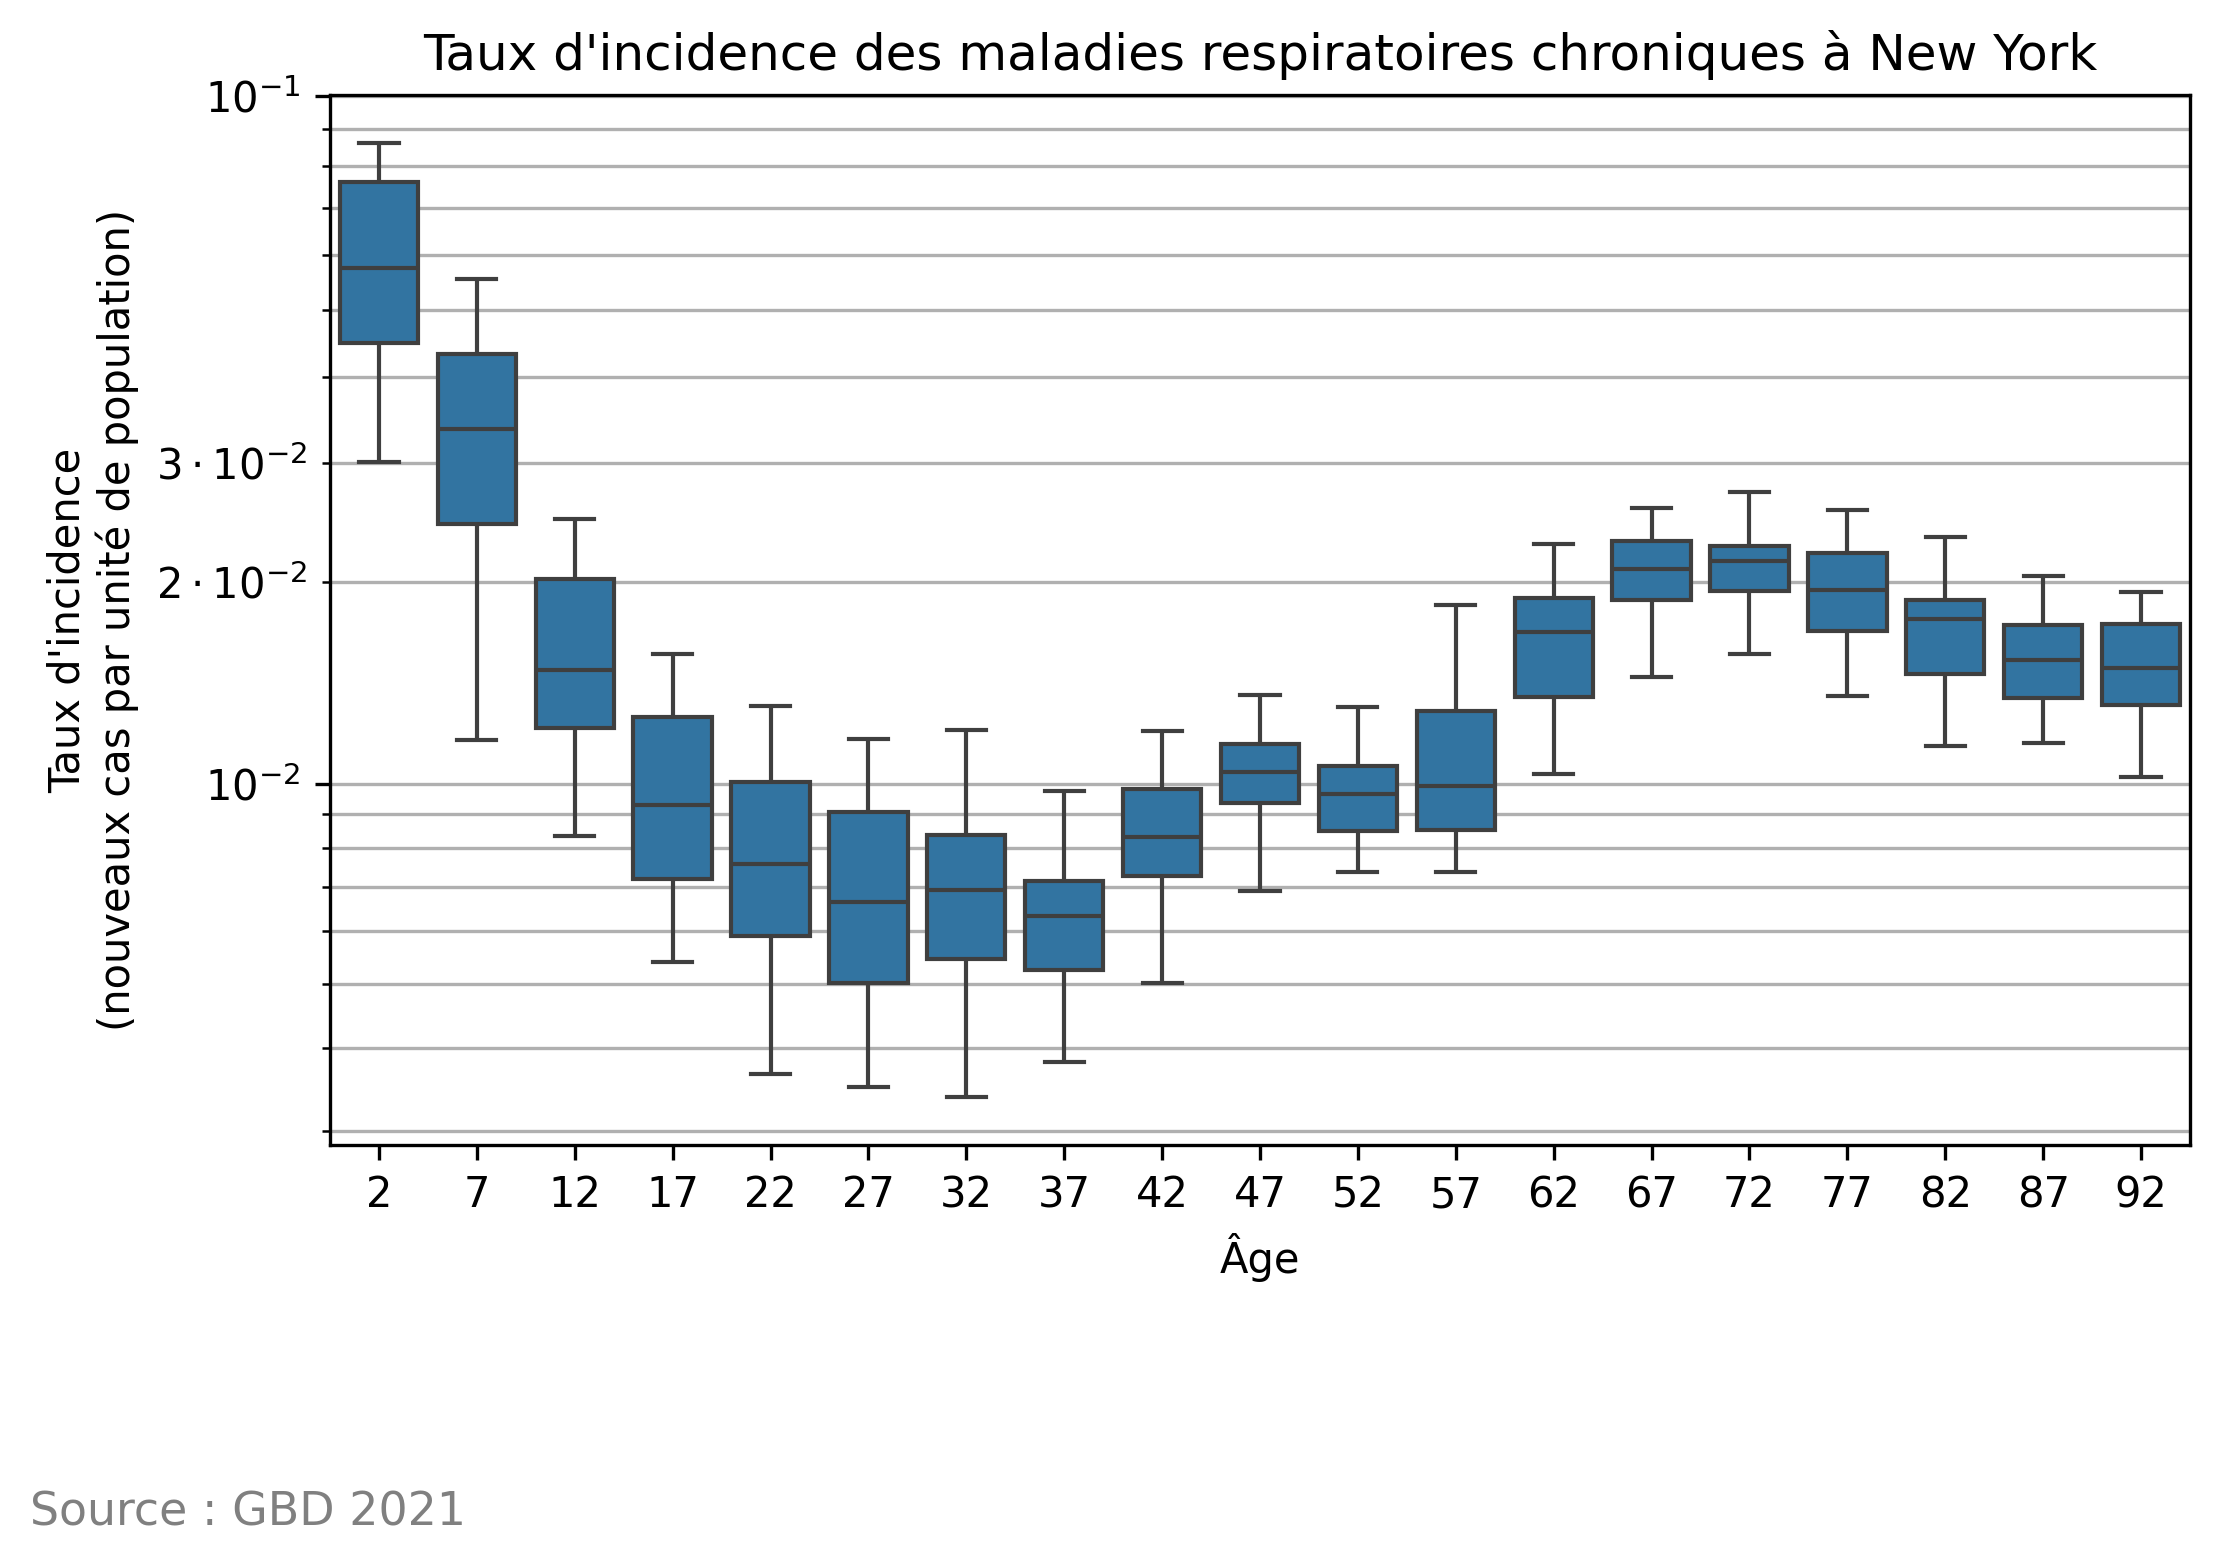
\includegraphics[width=1\textwidth]{images/incidence_new_york.png}
	\caption{Taux d'incidence (par unité de population) à New York. L'échelle des ordonnées est logit.}
	\label{fig:newyork-incidence}
\end{figure}

La figure~\ref{fig:newyork-incidence} suggère qu’une relation de forme cubique lie le taux d'incidence à l'âge. Le présent chapitre se propose de formaliser, vérifier puis généraliser cette observation à l'ensemble des États des États-Unis.


\section{Méthodologie statistique}

\subsection{Modèle de régression robuste}
l'objectif de cette section est de décrire comment nous relions l'incidence (par tranche d'âge) à l'incidence globale (tous âges confondus), tout en tenant compte de l'effet de l'âge de façon robuste aux observations atypiques (ou \emph{outliers}). 

\subsubsection*{Formulation du modèle}
Pour chaque groupe d'âge (dont l'âge moyen est $a$), on dispose d'une valeur d'incidence $i_a$, ainsi que d'une incidence globale $i_{\mathrm{globale}}$ (tous âges confondus). Les deux valeurs sont exprimées pour 100\,000 personnes. En notant
\[
\text{logit}(x) \;=\; \log\!\Bigl(\frac{x}{100000 - x}\Bigr),
\]
nous adoptons le modèle suivant à chaque itération :
\[
\text{logit}(i_a) 
\;=\; \alpha \;+\; 
\beta_0 \, \text{logit}\bigl(i_{\mathrm{globale}}\bigr) 
\;+\; \beta_1 \, a \;+\; \beta_2\,a^2 \;+\; \beta_3\,a^3 \;+\; \varepsilon,
\]
où $\alpha, \beta_0, \beta_1, \beta_2$ et $\beta_3$ sont les coefficients à estimer. Le choix de la fonction \(\text{logit}\) s'explique par la nature proportionnelle de l'incidence : en transformant l'incidence par \(\log\!\bigl(\frac{i_a}{100000 - i_a}\bigr)\), on évite le problème de valeurs extrêmes (taux extrêmement faibles ou très élevés) et on linearise mieux la relation avec l'âge.

\subsubsection*{Régression robuste avec la perte de Huber}
Le terme aléatoire \(\varepsilon\) est supposé suivre un modèle «~hubérisé~», c’est-à-dire que la \emph{fonction de perte} utilisée dans l'ajustement du modèle n'est pas simplement la somme des carrés des résidus (comme dans la régression linéaire classique), mais la \emph{perte de Huber}. 

\begin{itemize}
	\item \textbf{Pourquoi la perte de Huber~?} 
	
	La fonction de perte de Huber est une combinaison de la perte quadratique (pour les petits résidus) et de la perte absolue (pour les grands résidus). Concrètement, lorsque l'écart entre la valeur prédite et la valeur observée est faible, le modèle se comporte comme une régression aux moindres carrés. En revanche, si cet écart est trop important (observations atypiques, erreurs de mesure importantes, etc.), la perte de Huber se comporte comme une perte absolue, limitant ainsi l'influence de ces valeurs extrêmes. 
	
	\[
	\rho_{\delta}(r) = 
	\begin{cases}
		\frac{1}{2} \, r^2 \quad &\text{si } |r| \leq \delta, \\
		\delta\,\bigl(|r| - \frac{\delta}{2}\bigr) \quad &\text{sinon,}
	\end{cases}
	\]
	où \(r\) désigne le résidu (écart entre la prédiction et l'observation) et \(\delta\) est un paramètre de coupure. La régression robuste via \texttt{RLM(..., M=HuberT())} utilise par défaut le \emph{tuning constant} $\delta = 1,345$.
	
	\item \textbf{Avantage principal~: robustesse} 
	
	Grâce à cette approche, les valeurs potentiellement aberrantes sont «~moins pénalisées~», ce qui rend l'estimation des coefficients \((\alpha, \beta_0, \beta_1, \beta_2, \beta_3)\) plus stable et moins sensible aux données atypiques.
\end{itemize}

\subsubsection*{Échantillonnage pour refléter l'incertitude}
l'incidence $i_a$ et l'incidence globale $i_{\mathrm{globale}}$ ne sont pas des valeurs fixes, mais plutôt comprises dans un intervalle d'incertitude \([\ell, u]\). Pour chaque itération :
\begin{enumerate}
	\item Nous échantillonnons aléatoirement $i_a$ dans \([\ell_a, u_a]\) et $i_{\mathrm{globale}}$ dans \([\ell_{\mathrm{all}}, u_{\mathrm{all}}]\) suivant une loi uniforme. 
	\item Nous appliquons la transformation logit puis ajustons le modèle via la perte de Huber pour estimer \(\alpha, \beta_0, \beta_1, \beta_2, \beta_3\).
	\item Nous stockons les coefficients estimés.
\end{enumerate}
En répétant cette opération un grand nombre de fois (typiquement plusieurs centaines ou milliers d'itérations), nous tenons compte de la variabilité due à l'estimation du taux d'incidence. Enfin, nous moyennons les coefficients estimés pour obtenir des valeurs centrales robustes, accompagnées d'intervalles de crédibilité (ou de confiance) reflétant la variabilité observée.

Cette procédure fournit ainsi une image plus complète de l'incertitude, contrairement à une seule estimation ponctuelle, tout en restant robuste aux observations extrêmes.


\subsection{Tests de normalité des coefficients}
À l'issue du processus d'itération décrit précédemment, nous obtenons, pour chaque État, un grand nombre d'estimations pour chacun des coefficients du modèle (\(\alpha\), \(\beta_0\), \(\beta_1\), \(\beta_2\), \(\beta_3\)). Afin d'évaluer si ces distributions de coefficients (issues des multiples échantillonnages) peuvent être raisonnablement considérées comme normales, nous recourons au test de Shapiro–Wilk.

Le test de Shapiro–Wilk (souvent abrégé en \emph{SW test}) vérifie la proximité d'un échantillon de données par rapport à une distribution normale de référence. Concrètement, il calcule un indice (\emph{statistique W}) qui compare l'ordre des observations dans l'échantillon à l'ordre théorique de valeurs provenant d'une distribution normale. 
\begin{itemize}
	\item l'\emph{hypothèse nulle} (\(H_0\)) stipule que les données sont issues d'une distribution normale.
	\item Une valeur de \(p\)-value élevée (généralement \(p \geq 0{,}05\)) indique qu’aucune preuve forte ne permet de rejeter l'hypothèse de normalité.
	\item À l'inverse, si la \(p\)-value est très faible (\(p<0{,}05\)), on conclut que les données s'éloignent significativement d'une distribution normale.
\end{itemize}

Le test de Shapiro–Wilk est souvent privilégié pour des échantillons de taille faible à modérée. Pour des très grands échantillons, même de faibles déviations par rapport à la normalité peuvent conduire à un rejet de l'hypothèse nulle, ce qui doit être interprété avec prudence.

\subsubsection*{Application à nos coefficients}
Pour chaque État, nous considérons le nuage de valeurs estimées pour un coefficient donné (par exemple, \(\beta_1\)). Nous appliquons le test de Shapiro–Wilk à cet échantillon :
\begin{enumerate}
	\item \textbf{Estimation du coefficient.} Nous collectons les estimations issues des multiples itérations (après les tirages dans \([\ell,u]\) et l'ajustement du modèle robuste). 
	\item \textbf{Calcul de la statistique du test.} Le test de Shapiro–Wilk produit la statistique \(W\) et la \emph{value p} associée.
	\item \textbf{Interprétation.} 
	\begin{itemize}
		\item \(p \geq 0{,}05\)~: aucune évidence pour rejeter l'hypothèse de normalité. Les estimations du coefficient peuvent être considérées comme approximativement normales.
		\item \(p < 0{,}05\)~: l'hypothèse de normalité est rejetée au seuil de 5\,\%. Les estimations présentent une ou plusieurs caractéristiques (asymétrie, queues épaisses, etc.) qui s'éloignent d'une distribution normale.
	\end{itemize}
\end{enumerate}

Ce diagnostic de normalité permet notamment de vérifier la validité d'hypothèses statistiques ultérieures (par exemple, la construction d'intervalles de confiance ou l'utilisation de tests paramétriques), et de justifier ou non l'emploi de méthodes complémentaires plus robustes. 


\section{Résultats}

\subsection{Distributions des valuers p}
Le tableau~\ref{tab:shapiro} présente les valeurs p du test de Shapiro--Wilk appliqué aux distributions des coefficients robustes (\(\alpha\), \(\beta_0\), \(\beta_1\), \(\beta_2\), \(\beta_3\)) pour chacun des 50~États et le District of Columbia. Chaque ligne du tableau correspond à un État et chaque colonne à l'un des coefficients estimés.

\begin{table}[H]
	\centering
	\caption{Résultats du test de Shapiro--Wilk (valeurs p) par État et par coefficient. Une valuer p supérieure à 0,05 indique qu’il n'existe pas de preuve suffisante pour rejeter l'hypothèse de normalité au seuil de 5\,\%. Source : GBD 2021.}
	\label{tab:shapiro}
	\scalebox{0.85}{\begin{tabular}{lrrrrr}
	\toprule
	& Constante & $\begin{array}{c}
		\text{Incidence}\\\text{(tous les âges)}
	\end{array}$  & Âge & Âge$^{2}$ & Âge$^{3}$ \\
	État &  &  &  &  &  \\
\midrule
Florida & 0.900262 & 0.719677 & 0.962169 & 0.563169 & 0.482713 \\
Indiana & 0.046227 & 0.026316 & 0.259308 & 0.373499 & 0.295557 \\
Arizona & 0.266231 & 0.200417 & 0.644828 & 0.928012 & 0.821360 \\
District of Columbia & 0.192110 & 0.315677 & 0.630271 & 0.908799 & 0.589787 \\
Virginia & 0.459928 & 0.451890 & 0.933773 & 0.750506 & 0.775443 \\
Minnesota & 0.035898 & 0.039665 & 0.979166 & 0.985214 & 0.902774 \\
Alabama & 0.789109 & 0.930856 & 0.098207 & 0.100775 & 0.195099 \\
Kentucky & 0.399275 & 0.317714 & 0.368874 & 0.272306 & 0.461826 \\
Wisconsin & 0.578989 & 0.294828 & 0.665907 & 0.473481 & 0.608763 \\
Louisiana & 0.286008 & 0.391046 & 0.882237 & 0.869540 & 0.548751 \\
Oregon & 0.420299 & 0.295518 & 0.226837 & 0.439856 & 0.556087 \\
Ohio & 0.603272 & 0.872154 & 0.561491 & 0.186139 & 0.166579 \\
Nevada & 0.150145 & 0.349179 & 0.198798 & 0.036677 & 0.029377 \\
Texas & 0.379894 & 0.268752 & 0.559649 & 0.578125 & 0.659767 \\
Mississippi & 0.693148 & 0.823702 & 0.653253 & 0.994191 & 0.962616 \\
Alaska & 0.193820 & 0.306439 & 0.928482 & 0.827019 & 0.829079 \\
Connecticut & 0.097959 & 0.155841 & 0.929510 & 0.947488 & 0.971022 \\
Georgia & 0.857730 & 0.806463 & 0.595895 & 0.335236 & 0.297994 \\
North Carolina & 0.469925 & 0.581799 & 0.751414 & 0.751692 & 0.895083 \\
Wyoming & 0.004778 & 0.005386 & 0.847914 & 0.675758 & 0.684384 \\
New Jersey & 0.026770 & 0.037915 & 0.749857 & 0.773758 & 0.583323 \\
Rhode Island & 0.016973 & 0.012016 & 0.864882 & 0.423398 & 0.400641 \\
Washington & 0.120665 & 0.140095 & 0.533588 & 0.873975 & 0.887788 \\
Missouri & 0.232014 & 0.294303 & 0.640803 & 0.396093 & 0.177082 \\
Vermont & 0.593869 & 0.585375 & 0.731438 & 0.545405 & 0.350779 \\
Massachusetts & 0.550541 & 0.464981 & 0.556817 & 0.425361 & 0.412623 \\
Maryland & 0.333188 & 0.322741 & 0.817402 & 0.522865 & 0.593523 \\
Utah & 0.416914 & 0.233968 & 0.500383 & 0.599504 & 0.668291 \\
South Carolina & 0.205609 & 0.155599 & 0.740327 & 0.624069 & 0.717434 \\
Michigan & 0.082893 & 0.144240 & 0.486778 & 0.947819 & 0.976748 \\
Kansas & 0.135763 & 0.142002 & 0.965683 & 0.890911 & 0.923332 \\
New Mexico & 0.406371 & 0.332559 & 0.382242 & 0.204714 & 0.358130 \\
Iowa & 0.939622 & 0.951580 & 0.968355 & 0.829809 & 0.806361 \\
New York & 0.091702 & 0.153574 & 0.941865 & 0.989753 & 0.824668 \\
Arkansas & 0.736346 & 0.929694 & 0.544431 & 0.838450 & 0.780760 \\
Delaware & 0.003730 & 0.009623 & 0.501311 & 0.840542 & 0.642348 \\
Pennsylvania & 0.167352 & 0.156111 & 0.010462 & 0.057079 & 0.249097 \\
Colorado & 0.166951 & 0.337884 & 0.350400 & 0.225930 & 0.348391 \\
Idaho & 0.610961 & 0.651126 & 0.836059 & 0.759192 & 0.843739 \\
West Virginia & 0.153072 & 0.400901 & 0.245878 & 0.482385 & 0.503756 \\
California & 0.546507 & 0.537487 & 0.623897 & 0.528192 & 0.316758 \\
Tennessee & 0.826333 & 0.619585 & 0.625040 & 0.206343 & 0.232872 \\
Oklahoma & 0.056913 & 0.057975 & 0.922941 & 0.883862 & 0.748928 \\
Montana & 0.874656 & 0.766501 & 0.724507 & 0.810860 & 0.796844 \\
Maine & 0.823682 & 0.986323 & 0.996607 & 0.650141 & 0.438621 \\
Illinois & 0.643275 & 0.646493 & 0.286435 & 0.130874 & 0.108143 \\
New Hampshire & 0.003858 & 0.003582 & 0.132991 & 0.702489 & 0.824263 \\
Nebraska & 0.122026 & 0.063810 & 0.927237 & 0.808858 & 0.725433 \\
North Dakota & 0.435265 & 0.360600 & 0.069065 & 0.166695 & 0.055921 \\
Hawaii & 0.897619 & 0.935712 & 0.948668 & 0.592383 & 0.290948 \\
South Dakota & 0.251898 & 0.328966 & 0.964662 & 0.785235 & 0.691936 \\
\bottomrule
\end{tabular}
}
\end{table}

Bien que ce tableau fournisse le détail complet, il est parfois difficile d'appréhender la distribution globale des valeurs p à travers une simple liste de nombres. Afin de faciliter l'interprétation, nous avons recours à une représentation graphique sous forme de \emph{diagramme en violon}, représentée à la figure~\ref{fig:shapiro-violin}.

\begin{figure}[H]
	\centering
	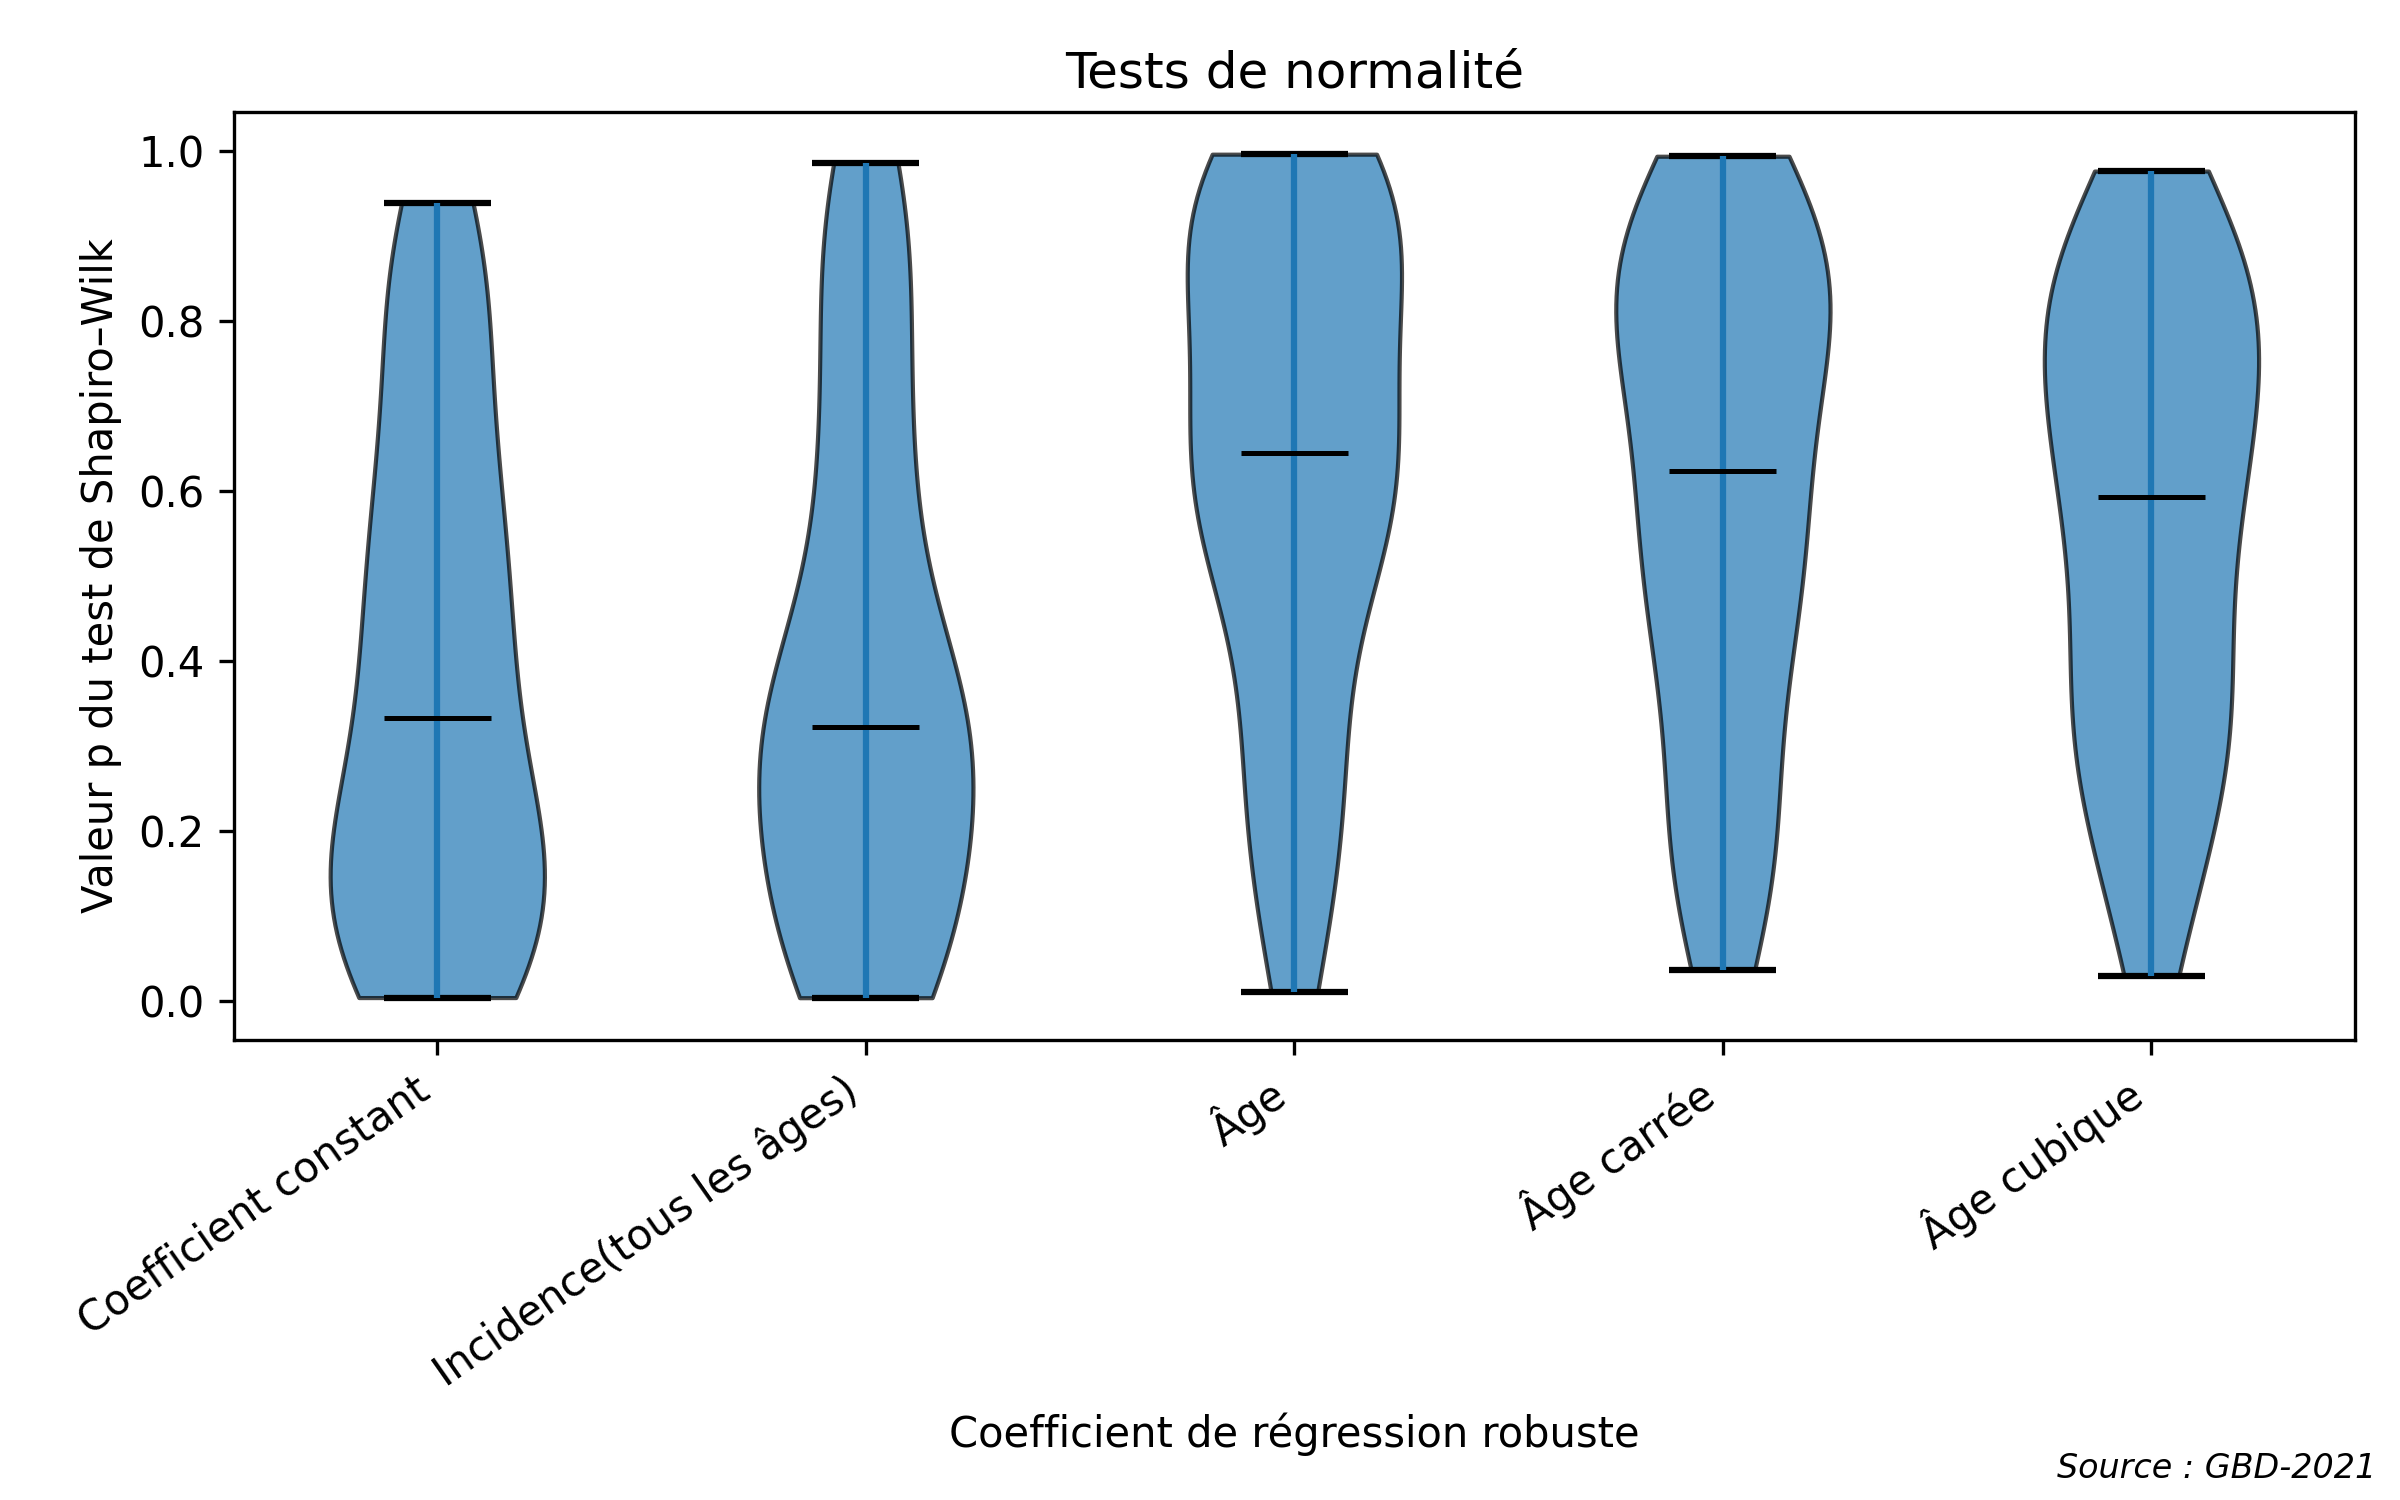
\includegraphics[width=1\textwidth]{images/shapiro_violin.png}
	\caption{Distribution en violon des valeurs p du test de Shapiro--Wilk, par coefficient (50~États et le District of Columbia). 
		Chaque colonne illustre la \emph{densité} (sur l'axe vertical) des valeurs p pour un coefficient donné. 
		La largeur du violon reflète la proportion de valeurs p à chaque niveau.}
	\label{fig:shapiro-violin}
\end{figure}

\subsubsection*{Interprétation et bonnes pratiques de visualisation}
\begin{itemize}
	\item \textbf{Diagrammes en violon}~: 
	\begin{enumerate}une boîte à moustaches central (indiquant la médiane et les quartiles) avec une courbe de densité symétrique autour de l'axe vertical. 
		\item Ils permettent de repérer rapidement les zones où les valeurs p sont les plus concentrées et d'identifier d'éventuelles valeurs extrêmes.
	\end{enumerate}
	
	\item \textbf{Seuil critique de 5\,\% (valeur p = 0,05)}~:  
	\begin{enumerate}
		\item Si la plupart des valeurs p se situent \emph{au-dessus} de 0,05, on ne rejette pas l'hypothèse de normalité pour la majorité des États.
		\item Si, au contraire, de nombreuses valeurs p sont \emph{inférieures} à 0,05, cela indique qu’on observe un écart significatif par rapport à la normalité dans plusieurs États.
	\end{enumerate}
	
	\item \textbf{Considérations pratiques}~:
	\begin{enumerate}
		\item \emph{Taille d'échantillon}~: Pour des séries de coefficients obtenus après de multiples itérations, la puissance du test de Shapiro--Wilk peut être élevée et conduire à un rejet de l'hypothèse de normalité pour de légères déviations.
		\item \emph{Variabilité entre les coefficients}~: Une différence notable dans la distribution des valeurs p entre deux coefficients peut suggérer que l'un est estimé de façon plus stable et plus conforme aux hypothèses de normalité que l'autre.
	\end{enumerate}
\end{itemize}

Dans l'ensemble, la combinaison du tableau~\ref{tab:shapiro} et du diagramme en violon (figure~\ref{fig:shapiro-violin}) offre une vision à la fois détaillée et synthétique de la normalité (ou non) des distributions de coefficients selon les 50~États et le District of Columbia. Cela permet ensuite de mieux apprécier la robustesse des inférences statistiques associées à chacun de ces coefficients.


\subsection{Estimateurs moyens des coefficients}

Au terme de nos multiples itérations, nous disposons, pour chaque État, d'un ensemble d'estimations pour les coefficients du modèle robuste : la constante \(\alpha\), l'effet global \(\beta_0\) (liant l'incidence par tranche d'âge à l'incidence globale), ainsi que les composantes linéaire (\(\beta_1\)), quadratique (\(\beta_2\)) et cubique (\(\beta_3\)) de l'âge. Nous calculons ensuite la moyenne de ces estimations, État par État, afin d'obtenir cinq \emph{estimateurs moyens} (un par coefficient).

\subsubsection*{Distribution globale des coefficients}
La figure~\ref{fig:violin-coeffs} illustre la distribution de ces coefficients moyens sur l'ensemble des 50~États et le District of Columbia, sous forme de diagrammes en violon. Chaque violon permet de repérer :
\begin{itemize}
	\item \textbf{La densité des valeurs}: la largeur du violon renseigne sur la concentration des valeurs autour de certaines zones.
	\item \textbf{La médiane et les quartiles}: visibles grâce à un marqueur central (ligne horizontale) indiquant la médiane, et parfois des traits indiquant les quartiles.
	\item \textbf{Les éventuelles valeurs extrêmes ou asymétries}: si la forme du violon est nettement allongée ou décalée, cela peut révéler une plus grande variabilité ou une asymétrie dans les estimations d'un coefficient.
\end{itemize}

\begin{figure}[H]
	\centering
	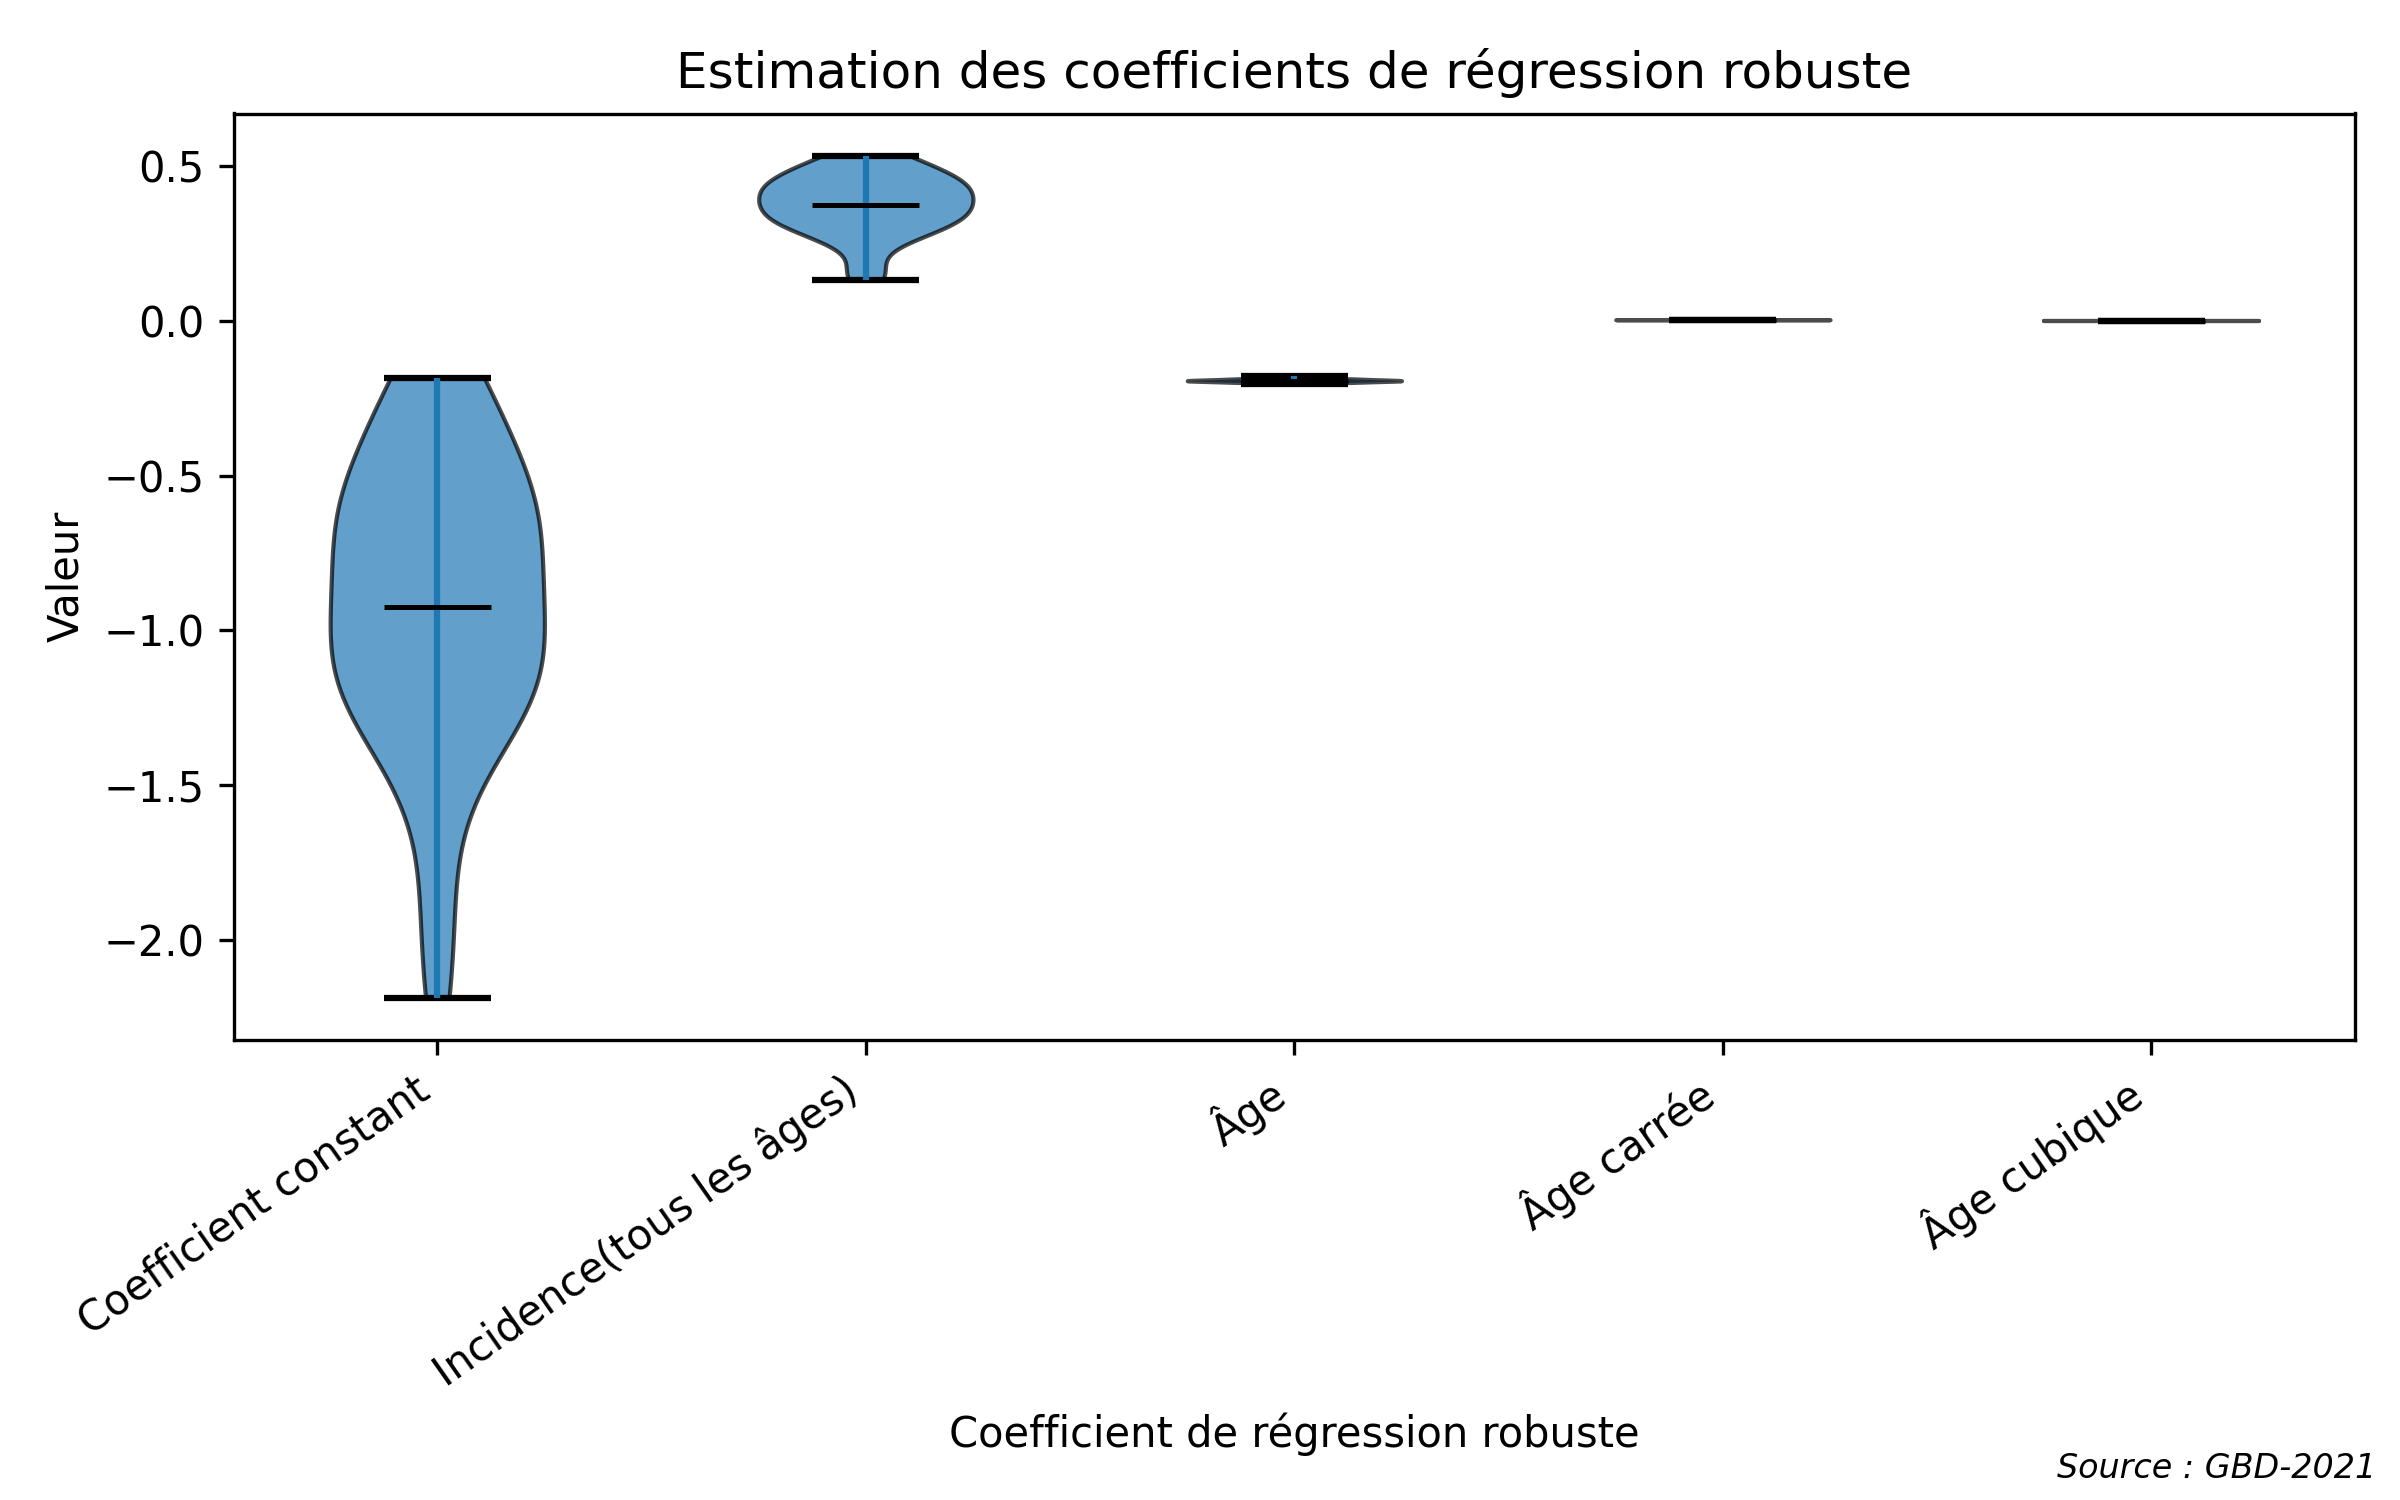
\includegraphics[width=1\textwidth]{images/violin_coefficients.png}
	\caption{Distribution en violon des coefficients moyens de la régression robuste, tous États confondus. 
		La largeur de chaque violon indique la densité estimée des valeurs à chaque niveau.}
	\label{fig:violin-coeffs}
\end{figure}

\subsubsection*{Tableau récapitulatif par État}
Pour une analyse plus détaillée, le tableau~\ref{tab:coeff-moy} ci-après répertorie ces coefficients moyens pour chaque État. Cette vue granulaire peut s'avérer pertinente, par exemple, si l'on souhaite comparer directement deux États voisins ou si l'on s'intéresse aux extrêmes (États pour lesquels les coefficients sont particulièrement élevés ou faibles).

\begin{table}[H]
	\centering
	\caption{Coefficients moyens du modèle robuste par État. Les valeurs présentées correspondent à la moyenne des estimations obtenues via les multiples itérations d'échantillonnage et d'ajustement (régression robuste). Source : GBD 2021.}
	\label{tab:coeff-moy}
	\scalebox{0.85}{\begin{tabular}{lrrrrr}
	\toprule
	& Constante & $\begin{array}{c}
	\text{Incidence}\\\text{(tous les âges)}
\end{array}$  & Âge & Âge$^{2}$ & Âge$^{3}$ \\
État &  &  &  &  &  \\
\midrule
Georgia & -0.671946 & 0.430326 & -0.198000 & 0.004449 & -0.000027 \\
Idaho & -1.965648 & 0.158865 & -0.190018 & 0.004262 & -0.000026 \\
Wisconsin & -1.222907 & 0.330755 & -0.184288 & 0.004086 & -0.000025 \\
Kansas & -0.781263 & 0.406307 & -0.196285 & 0.004359 & -0.000027 \\
Alaska & -1.884132 & 0.151040 & -0.190711 & 0.004134 & -0.000024 \\
District of Columbia & -1.346955 & 0.269259 & -0.179566 & 0.003815 & -0.000023 \\
New Hampshire & -0.838015 & 0.385153 & -0.194291 & 0.004313 & -0.000026 \\
Maine & -0.545244 & 0.440159 & -0.198476 & 0.004388 & -0.000027 \\
Nevada & -1.225596 & 0.304739 & -0.190018 & 0.004194 & -0.000025 \\
Arkansas & -1.151253 & 0.351523 & -0.185039 & 0.004144 & -0.000025 \\
New Jersey & -0.204345 & 0.514698 & -0.200054 & 0.004410 & -0.000027 \\
Connecticut & -0.205225 & 0.513576 & -0.198130 & 0.004352 & -0.000026 \\
Missouri & -0.544167 & 0.460457 & -0.193552 & 0.004315 & -0.000026 \\
Colorado & -0.971400 & 0.343362 & -0.199803 & 0.004422 & -0.000027 \\
Rhode Island & -0.418249 & 0.469570 & -0.195052 & 0.004290 & -0.000026 \\
Nebraska & -1.120373 & 0.366173 & -0.186783 & 0.004204 & -0.000026 \\
Florida & -0.492848 & 0.471961 & -0.194814 & 0.004349 & -0.000027 \\
Mississippi & -1.106534 & 0.377411 & -0.186475 & 0.004237 & -0.000026 \\
Vermont & -1.108899 & 0.326219 & -0.192628 & 0.004250 & -0.000026 \\
Louisiana & -1.188533 & 0.331680 & -0.192397 & 0.004349 & -0.000027 \\
Maryland & -0.623663 & 0.434829 & -0.192420 & 0.004261 & -0.000026 \\
Oregon & -1.321628 & 0.297876 & -0.186333 & 0.004138 & -0.000025 \\
Pennsylvania & -0.202719 & 0.529016 & -0.193086 & 0.004259 & -0.000026 \\
Delaware & -0.614979 & 0.416641 & -0.198489 & 0.004369 & -0.000027 \\
Illinois & -0.962975 & 0.374315 & -0.187745 & 0.004173 & -0.000025 \\
Kentucky & -0.516919 & 0.468000 & -0.193981 & 0.004348 & -0.000027 \\
West Virginia & -0.197746 & 0.525634 & -0.195545 & 0.004340 & -0.000026 \\
Massachusetts & -0.896073 & 0.358072 & -0.196900 & 0.004354 & -0.000027 \\
New York & -0.267371 & 0.513713 & -0.186473 & 0.004108 & -0.000025 \\
Alabama & -0.566789 & 0.459257 & -0.193196 & 0.004316 & -0.000026 \\
California & -1.249773 & 0.290689 & -0.198156 & 0.004413 & -0.000027 \\
South Dakota & -1.408039 & 0.288593 & -0.191311 & 0.004276 & -0.000026 \\
Montana & -1.275156 & 0.293896 & -0.193819 & 0.004304 & -0.000026 \\
New Mexico & -0.969591 & 0.347537 & -0.192991 & 0.004247 & -0.000026 \\
Ohio & -0.329737 & 0.515963 & -0.190680 & 0.004256 & -0.000026 \\
Utah & -2.111485 & 0.149834 & -0.177633 & 0.003913 & -0.000023 \\
Tennessee & -0.829140 & 0.420391 & -0.188904 & 0.004265 & -0.000026 \\
Texas & -0.768053 & 0.393132 & -0.204142 & 0.004559 & -0.000028 \\
Arizona & -0.912814 & 0.360985 & -0.193649 & 0.004295 & -0.000026 \\
Indiana & -0.476412 & 0.469788 & -0.195229 & 0.004352 & -0.000027 \\
Michigan & -0.482946 & 0.466191 & -0.192444 & 0.004259 & -0.000026 \\
North Carolina & -0.785923 & 0.424856 & -0.191566 & 0.004322 & -0.000027 \\
Minnesota & -1.238576 & 0.309178 & -0.195062 & 0.004279 & -0.000026 \\
South Carolina & -0.572408 & 0.476576 & -0.186667 & 0.004199 & -0.000026 \\
Virginia & -0.833369 & 0.390105 & -0.193818 & 0.004322 & -0.000026 \\
Hawaii & -1.438490 & 0.238511 & -0.187950 & 0.004071 & -0.000024 \\
North Dakota & -1.158724 & 0.323574 & -0.194520 & 0.004304 & -0.000026 \\
Wyoming & -1.622545 & 0.218802 & -0.191542 & 0.004249 & -0.000026 \\
Iowa & -1.186115 & 0.358169 & -0.186266 & 0.004193 & -0.000026 \\
Washington & -1.344826 & 0.298453 & -0.188853 & 0.004199 & -0.000025 \\
Oklahoma & -0.692055 & 0.415745 & -0.197038 & 0.004394 & -0.000027 \\
\bottomrule
\end{tabular}
}
\end{table}

\subsection{Visualisation géographique des coefficients}
La répartition spatiale des coefficients moyens est représentée sur les cartes choroplèthes ci-dessous, selon la palette de couleurs \(\texttt{Viridis}\), qui est \emph{color-blind friendly} et met en évidence les variations de valeur de façon progressive. Chaque carte met l'accent sur l'un des cinq coefficients. 

\vspace{1em}
\subsubsection{Carte de la constante (\(\alpha\)):}

\begin{figure}[H]
	\centering
	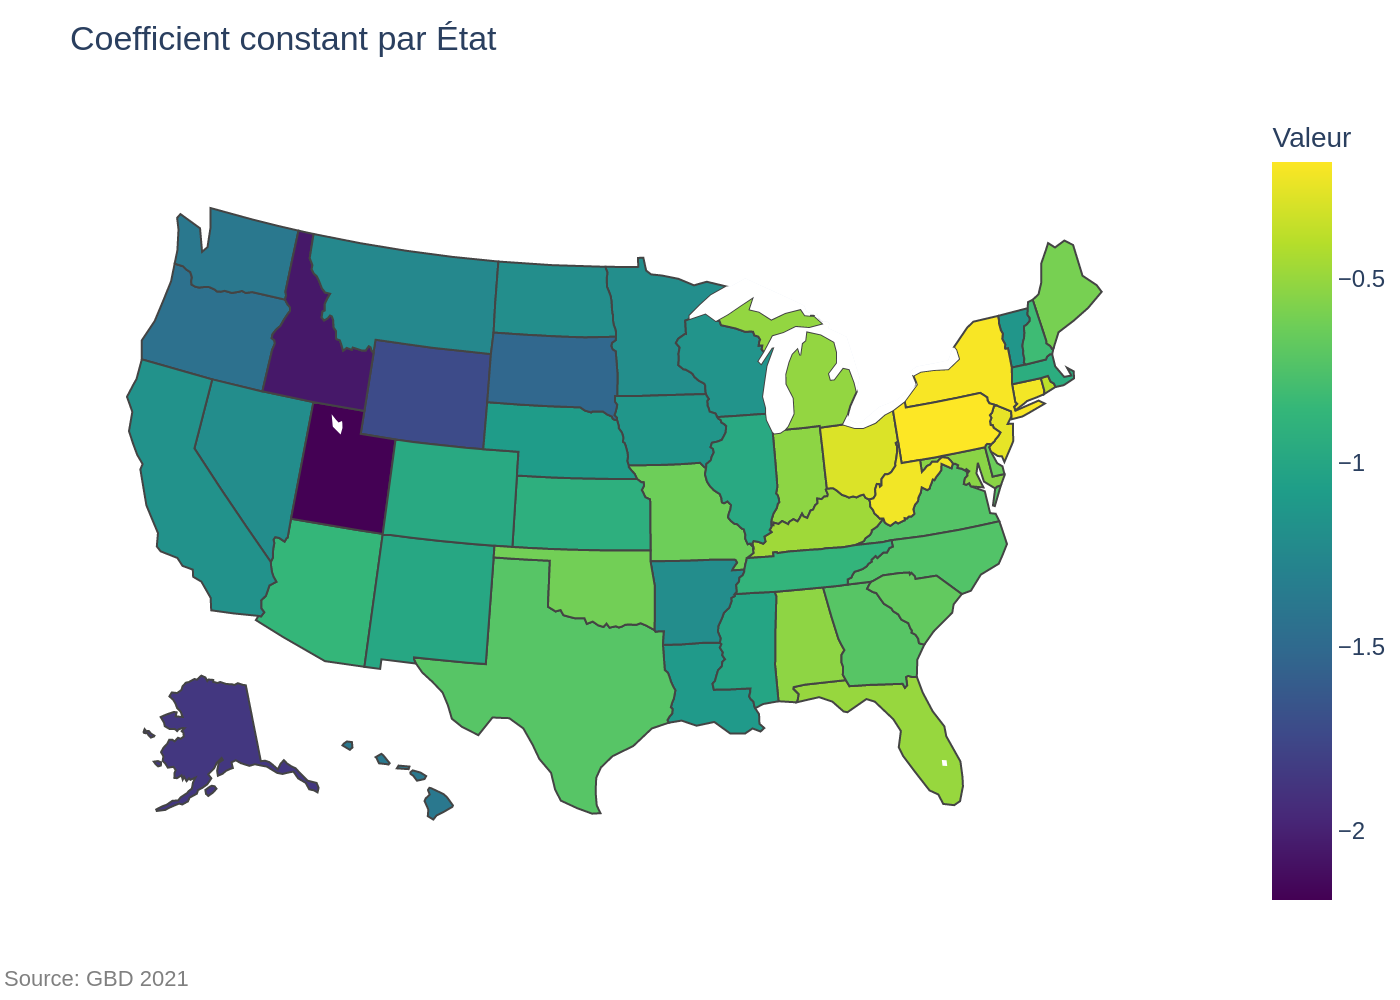
\includegraphics[width=1\textwidth]{images/map_const.png}
	\caption{Valeurs moyennes de \(\alpha\) (coefficient constant) par État. 
		Plus la couleur est foncée, plus la valeur estimée est élevée.}
\end{figure}

\subsubsection{Carte du coefficient \(\beta_0\) (incidence globale):}

\begin{figure}[H]
	\centering
	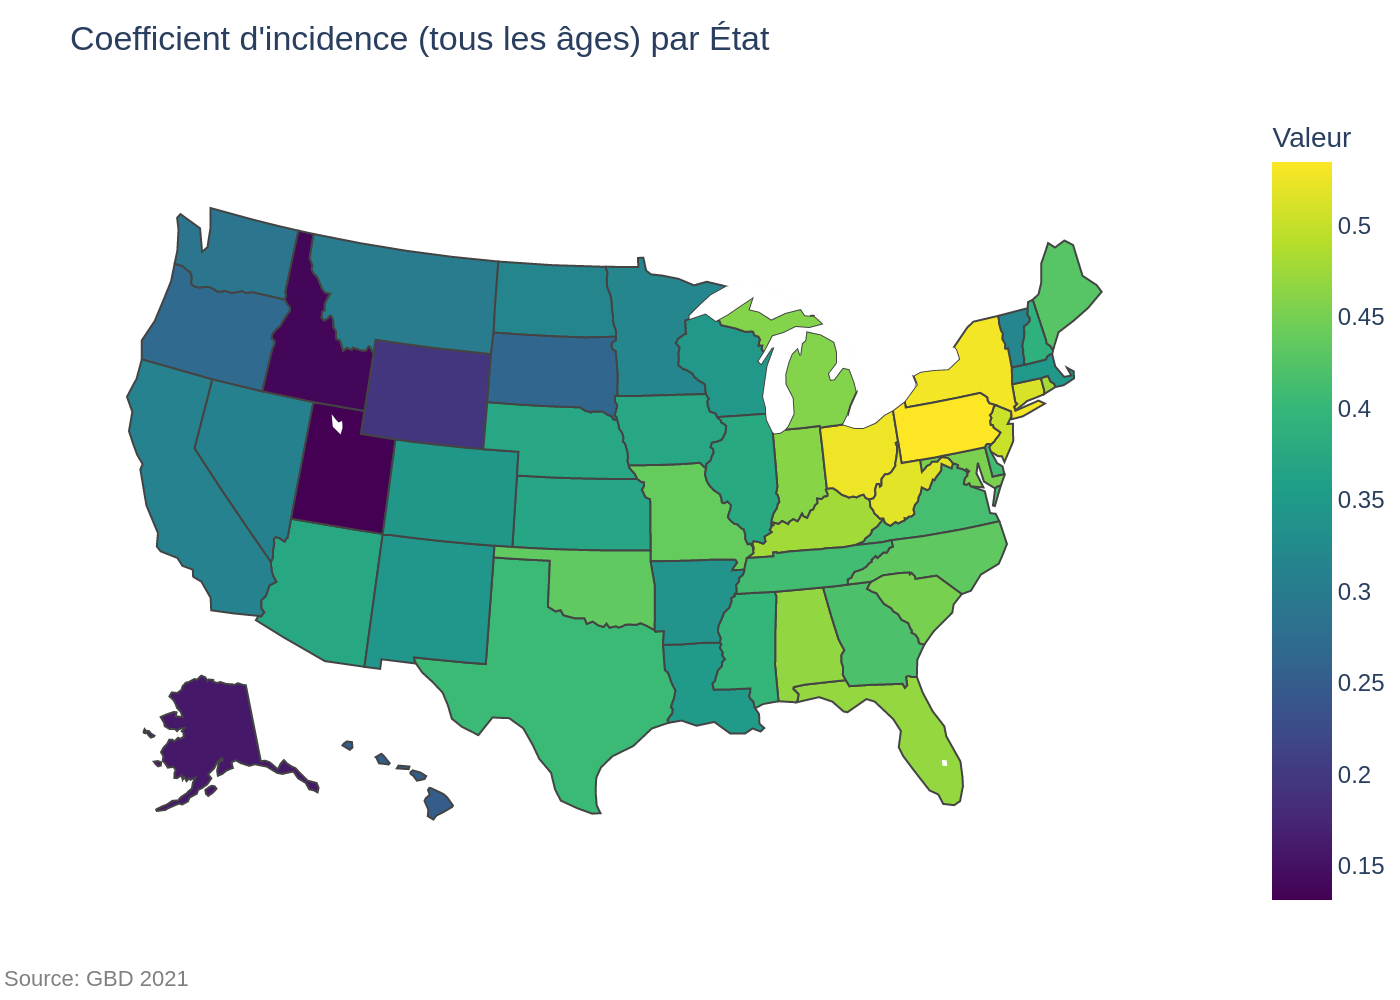
\includegraphics[width=1\textwidth]{images/map_incidence_all.png}
	\caption{Valeurs moyennes de \(\beta_0\) (log-odds de l'incidence globale) par État. 
		Les zones plus foncées indiquent un effet global plus prononcé de l'incidence.}
\end{figure}

\subsubsection{Carte du coefficient \(\beta_1\) (âge):}

\begin{figure}[H]
	\centering
	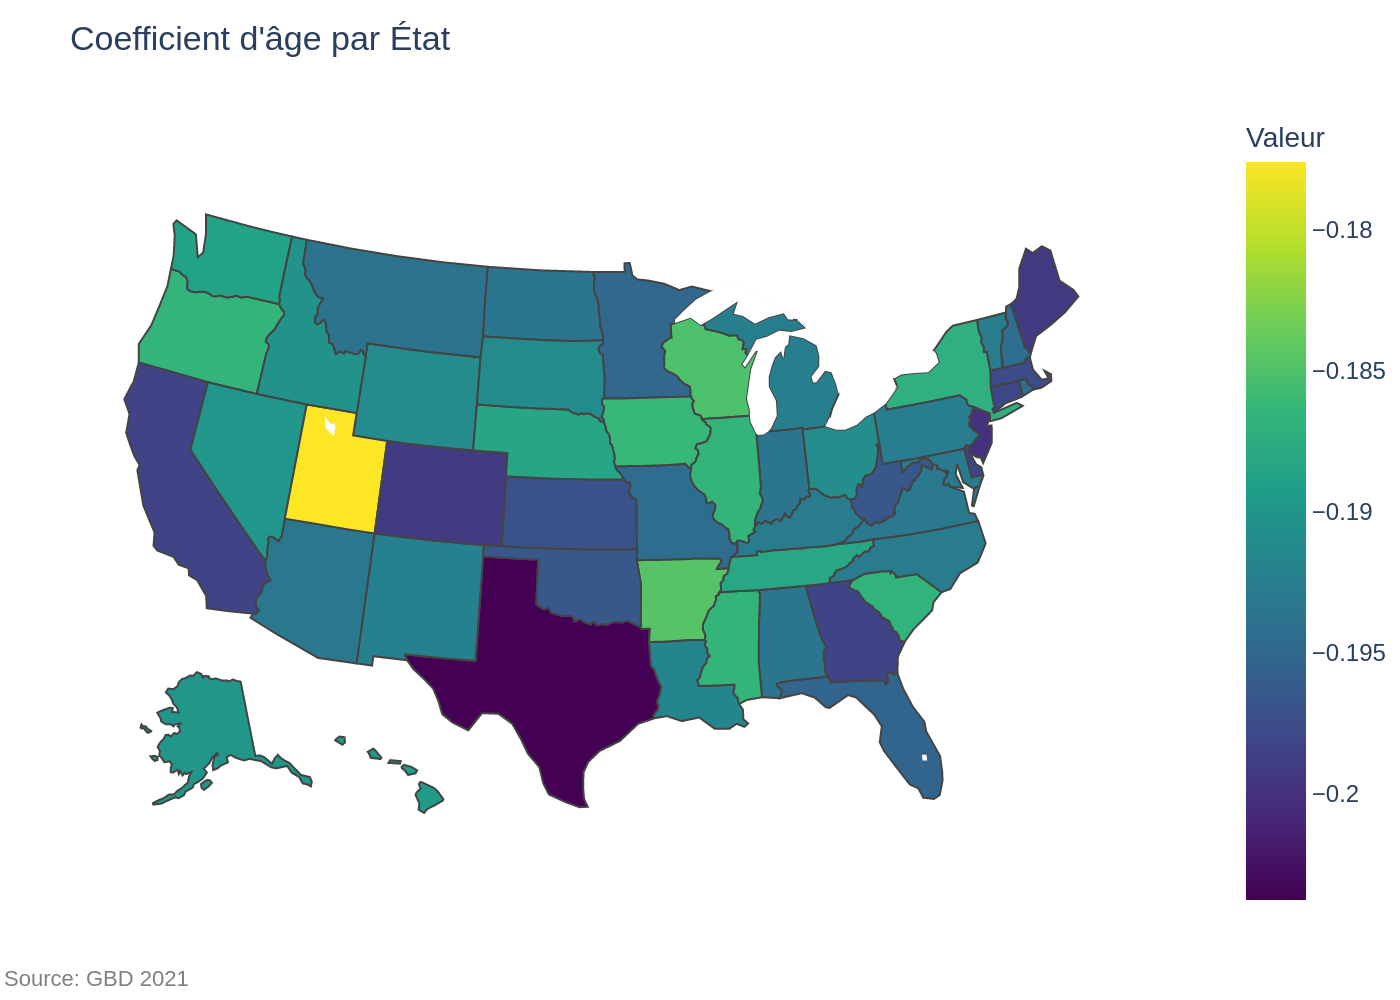
\includegraphics[width=1\textwidth]{images/map_age.png}
	\caption{Valeurs moyennes de \(\beta_1\) (terme linéaire en âge) par État.}
\end{figure}

\subsubsection{Carte du coefficient \(\beta_2\) (âge au carré):}

\begin{figure}[H]
	\centering
	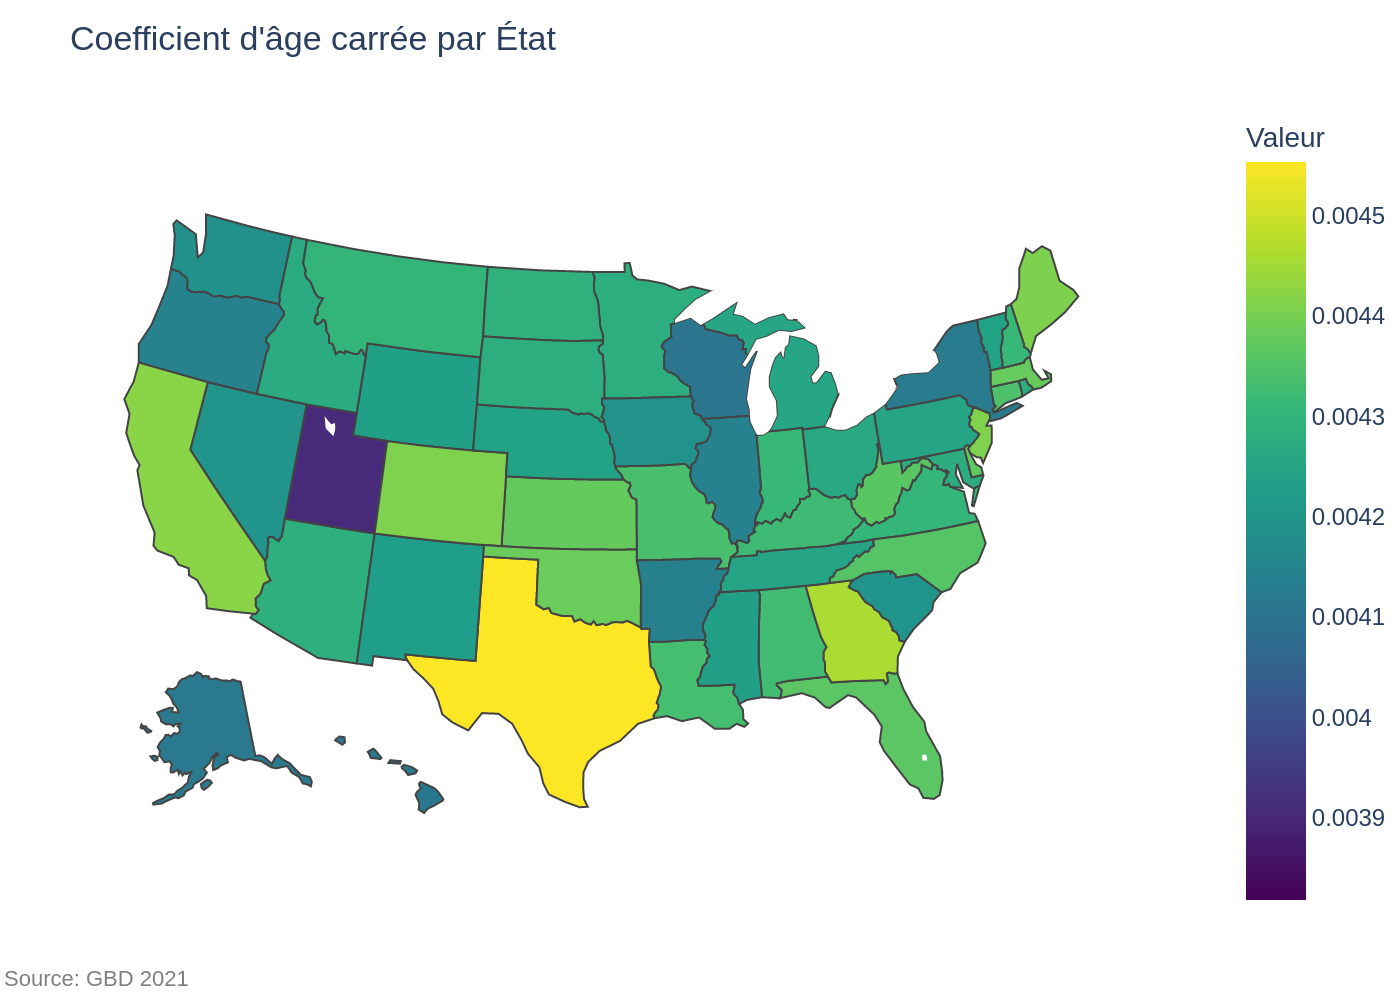
\includegraphics[width=1\textwidth]{images/map_age2.png}
	\caption{Valeurs moyennes de \(\beta_2\) (terme quadratique) par État.}
\end{figure}

\subsubsection{Carte du coefficient \(\beta_3\) (âge au cube):}

\begin{figure}[H]
	\centering
	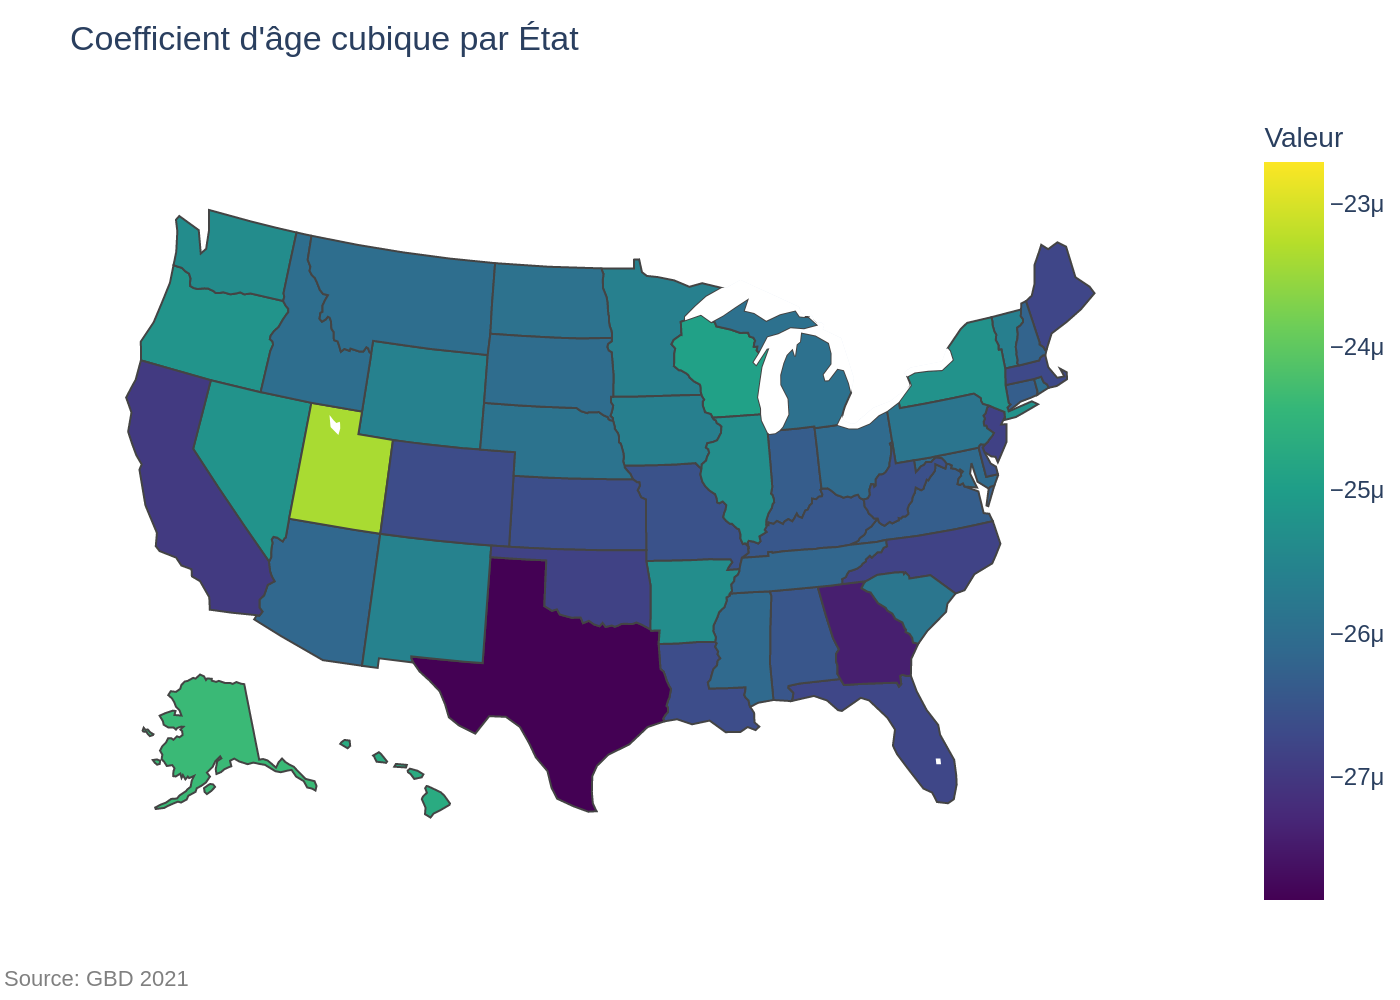
\includegraphics[width=1\textwidth]{images/map_age3.png}
	\caption{Valeurs moyennes de \(\beta_3\) (terme cubique) par État.}
\end{figure}

\section{Qualité prédictive du modèle : synthèse par État}

\subsubsection*{Paramètres de la validation croisée}
La qualité de prédiction a été évaluée par \textbf{validation croisée à $k=10$ plis}
(\emph{10-fold cross-validation}), avec permutation préalable des données
(\texttt{shuffle = True}) et \textbf{graine aléatoire fixée à 42} afin de garantir la
reproductibilité des résultats.\footnote{En pratique, nous utilisons la classe
	\texttt{KFold} de \textsc{scikit-learn} (\texttt{n\_splits = 10,
		random\_state = 42}).}  
Le critère d’évaluation est la
\textbf{sMAPE}\,(Symmetrical Mean Absolute Percentage Error), définie pour
chaque observation $(y, \hat y)$ par
\[
\mathrm{sMAPE} \;=\;
\frac{|\,y - \hat y\,|}{\tfrac{|y| + |\hat y|}{2}}\;\times 100~\%.
\]

Un faible terme $\varepsilon = 10^{-8}$ est ajouté au dénominateur pour éviter toute division par zéro.

Cette métrique, bornée entre $0$ et $100~\%$, est insensible aux valeurs nulles
et pénalise de façon symétrique les sure- et sous-estimations.  Pour chaque
État et chaque pli, le modèle robuste à perte de Huber
est ré-estimé puis évalué, produisant ainsi $10$ valeurs de sMAPE par
territoire.

\subsubsection*{Statistiques récapitulatives}
Le tableau~\ref{tab:smape-states} rassemble, pour chacun des 50 États et le
District of Columbia, trois indicateurs issus de ces $10$ valeurs :

\begin{enumerate}
	\item le \emph{minimum} : meilleure performance observée ;
	\item la \emph{moyenne} : performance typique ;
	\item le \emph{maximum} : pire performance observée.
\end{enumerate}

Dans l’ensemble, la \textbf{sMAPE moyenne se situe entre 4 \% et 7 \%}, ce qui
traduit une excellente adéquation du modèle robuste ; même dans les cas les
plus défavorables la sMAPE reste modérée (\emph{maxima} rarement au-delà de
10 \%).

\newpage
\begin{table}[H]
	\centering
	\caption{Statistiques sMAPE (minimum, moyenne, maximum) par État.
		$k = 10$ plis, graine = 42, métrique = sMAPE.
		Source : GBD 2021.}
	\label{tab:smape-states}
	\scalebox{0.85}{\begin{tabular}{lrrr}
\toprule
 & smape (min) & smape (moyenne) & smape (max) \\
État &  &  &  \\
\midrule
Mississippi & 3.44 & 4.37 & 5.32 \\
Arkansas & 3.62 & 4.40 & 5.38 \\
Florida & 3.72 & 4.44 & 5.55 \\
Missouri & 3.93 & 4.48 & 5.00 \\
South Dakota & 3.53 & 4.56 & 5.77 \\
Ohio & 3.79 & 4.59 & 5.35 \\
Indiana & 4.12 & 4.60 & 5.03 \\
Maryland & 3.82 & 4.62 & 5.50 \\
Tennessee & 4.27 & 4.63 & 5.45 \\
North Carolina & 3.94 & 4.72 & 5.67 \\
Alaska & 4.06 & 4.75 & 5.47 \\
Iowa & 4.31 & 4.76 & 5.51 \\
Wyoming & 3.76 & 4.76 & 6.27 \\
West Virginia & 4.17 & 4.76 & 5.56 \\
Nebraska & 4.13 & 4.77 & 5.89 \\
South Carolina & 3.72 & 4.77 & 5.70 \\
Georgia & 3.90 & 4.77 & 5.37 \\
Wisconsin & 3.76 & 4.77 & 5.44 \\
Kentucky & 4.15 & 4.78 & 5.49 \\
Louisiana & 3.87 & 4.78 & 5.35 \\
Nevada & 4.15 & 4.78 & 6.20 \\
Maine & 4.42 & 4.80 & 5.45 \\
Kansas & 4.22 & 4.81 & 5.44 \\
Washington & 4.03 & 4.82 & 5.92 \\
Alabama & 4.09 & 4.84 & 5.44 \\
Oklahoma & 4.05 & 4.85 & 5.52 \\
Michigan & 4.25 & 4.86 & 5.45 \\
Vermont & 3.90 & 4.87 & 6.09 \\
Utah & 4.23 & 4.88 & 5.56 \\
Rhode Island & 4.28 & 4.88 & 5.67 \\
New Hampshire & 4.12 & 4.89 & 5.62 \\
California & 4.05 & 4.89 & 5.50 \\
Illinois & 3.77 & 4.91 & 5.71 \\
Montana & 4.05 & 4.92 & 5.73 \\
Massachusetts & 4.24 & 4.93 & 6.02 \\
Delaware & 4.02 & 4.95 & 5.85 \\
Idaho & 4.27 & 4.97 & 5.92 \\
Arizona & 4.15 & 4.99 & 5.65 \\
Pennsylvania & 4.42 & 4.99 & 5.84 \\
Texas & 4.36 & 5.02 & 6.27 \\
Minnesota & 4.17 & 5.04 & 6.31 \\
District of Columbia & 4.49 & 5.05 & 5.81 \\
Virginia & 4.21 & 5.06 & 5.58 \\
Hawaii & 4.43 & 5.06 & 6.39 \\
North Dakota & 4.28 & 5.07 & 6.68 \\
Oregon & 4.54 & 5.10 & 5.90 \\
Connecticut & 4.24 & 5.10 & 5.84 \\
New Mexico & 4.27 & 5.11 & 5.92 \\
Colorado & 4.29 & 5.13 & 5.87 \\
New Jersey & 4.55 & 5.25 & 5.89 \\
New York & 4.83 & 5.36 & 6.33 \\
\bottomrule
\end{tabular}
}
\end{table}
\newpage

\begin{figure}[H]
	\centering
	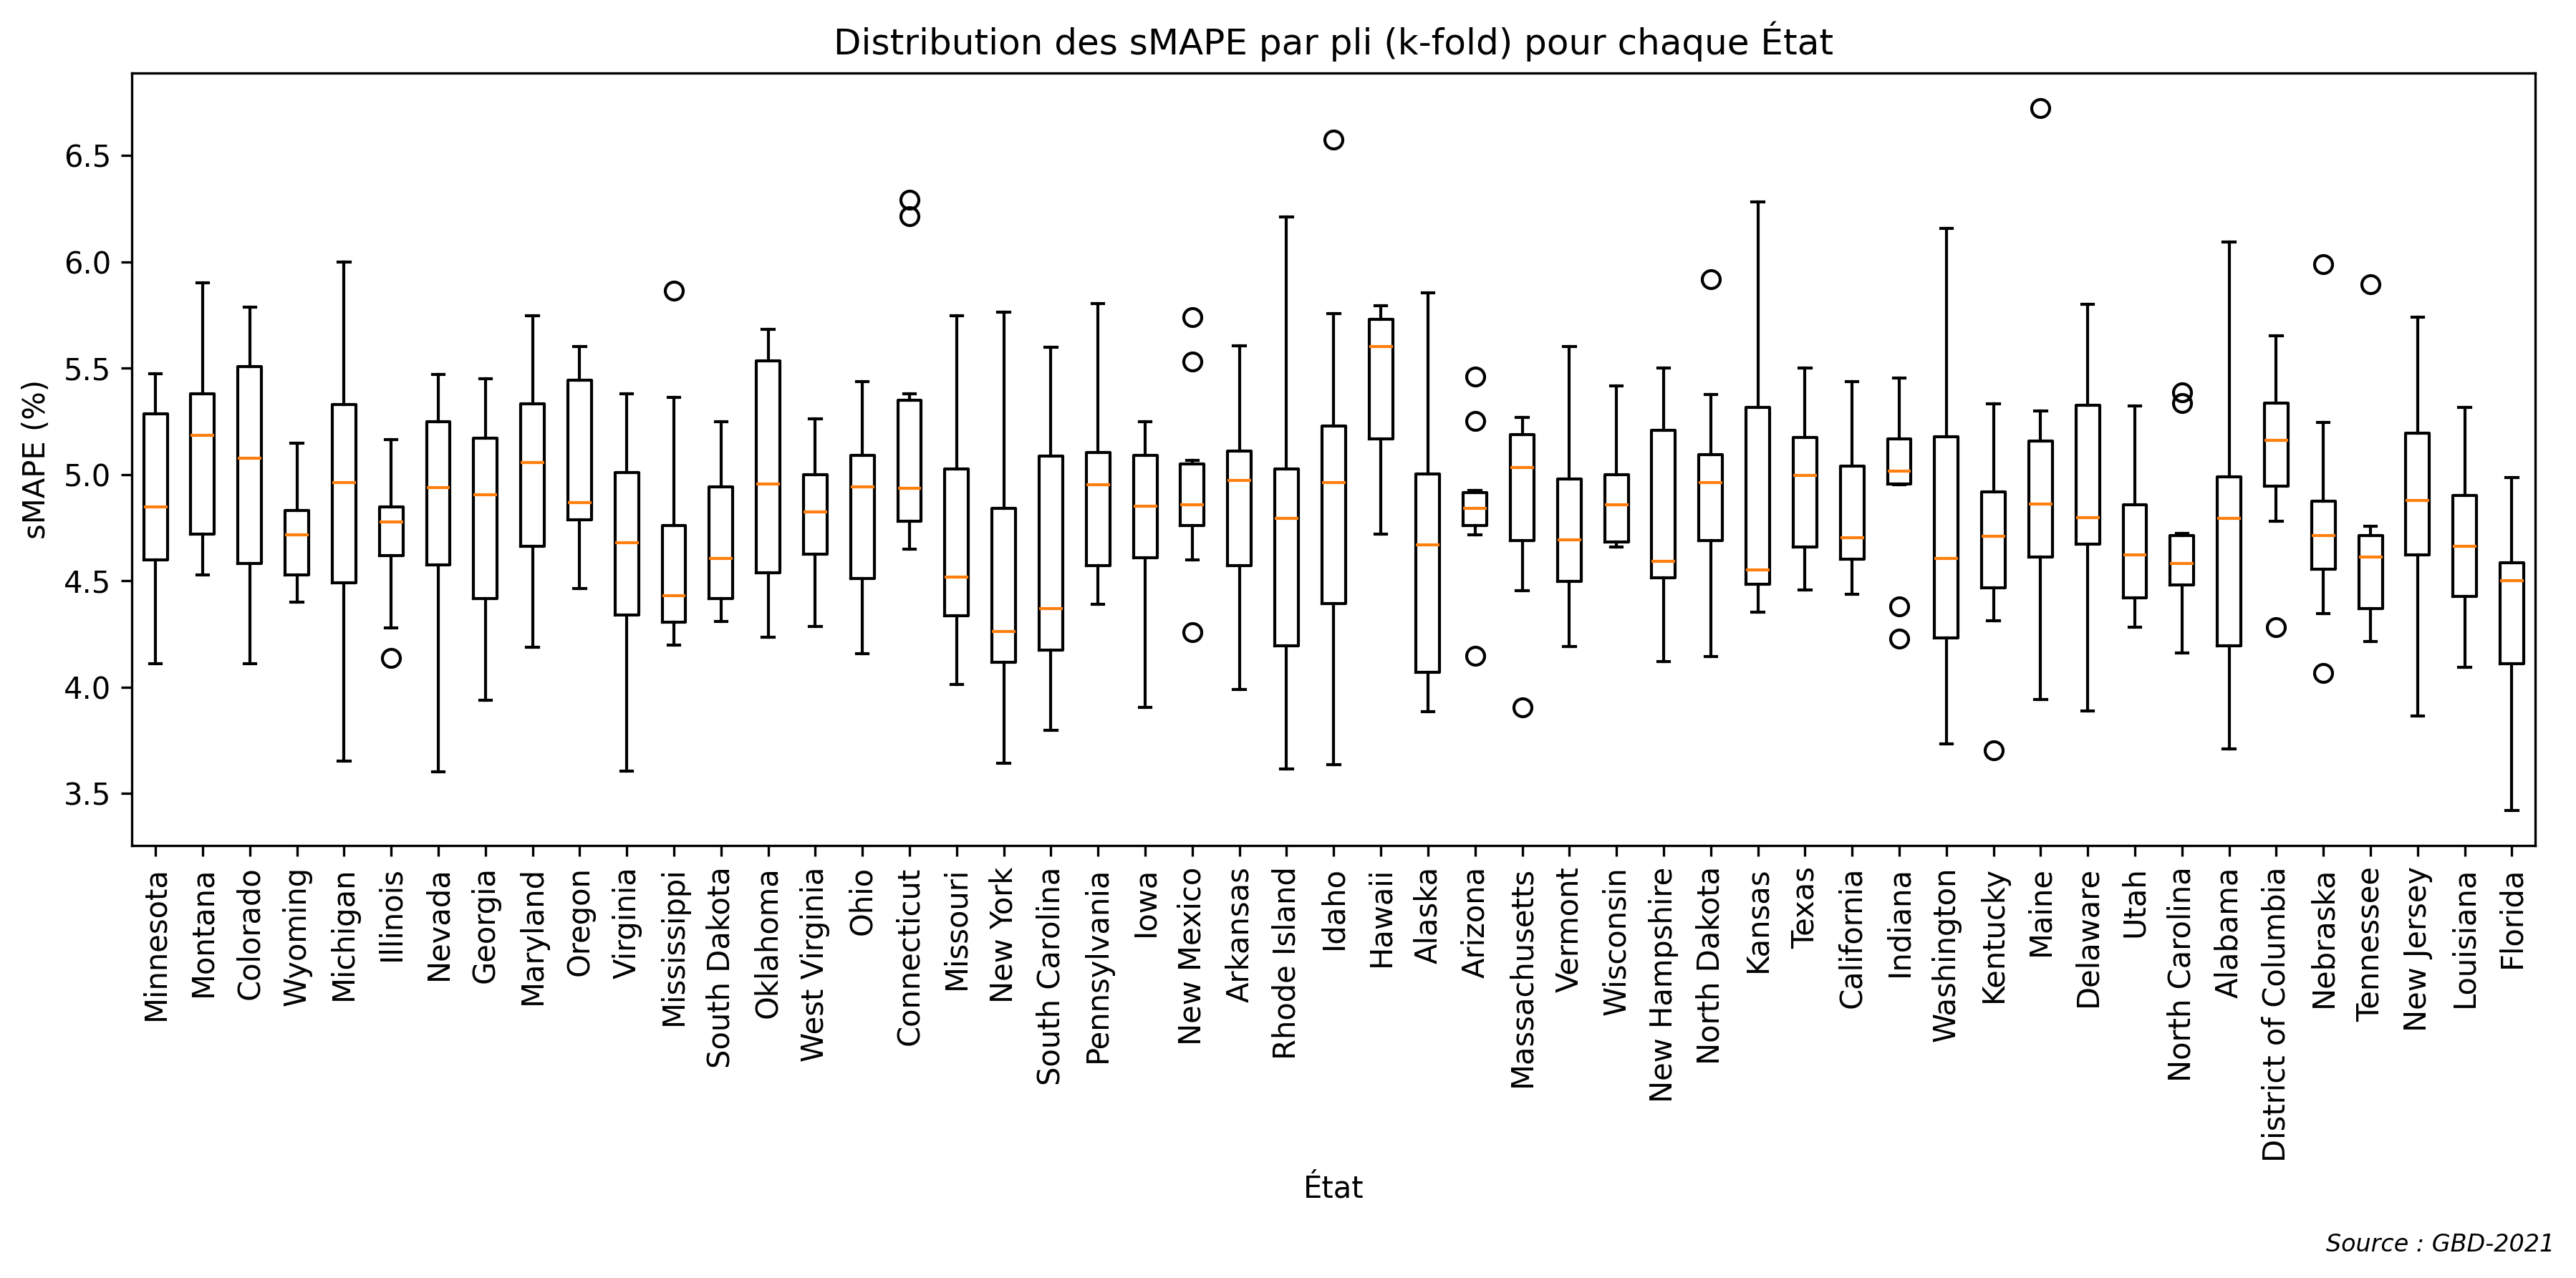
\includegraphics[width=1\textwidth]{images/boxplot_smape_etats.png}
	\caption{Distribution des sMAPE par pli ($k=10$) pour chaque État.}
	\label{fig:smape-boxplot}
\end{figure}

La figure~\ref{fig:smape-boxplot} apporte une vision graphique de la dispersion
des sMAPE :

\begin{itemize}
	\item Les boîtes, centrées autour d’une médiane proche de 5 \%, sont
	généralement compactes, signe d’une variabilité limitée entre plis.  
	\item Quelques moustaches plus étendues (valeurs hors-quartile) indiquent,
	pour certains États, une sensibilité accrue au découpage aléatoire des
	données, sans toutefois atteindre des niveaux d’erreur critiques.  
\end{itemize}

Avec un schéma de validation croisée rigoureux ($k=10$, graine fixée) et une
métrique relative stricte (sMAPE), la régression linéaire robuste à perte de
Huber montre une \textbf{performance stable et élevée} sur l’ensemble des
États.  Les écarts territoriaux observés restent modestes et n'affectent pas
les conclusions globales présentées dans les sections suivantes.

\section{Discussion}

Les résultats obtenus éclairent la relation entre l'incidence des maladies respiratoires chroniques et l'âge, tout en révélant des disparités géographiques au sein des États-Unis. Dans cette section, nous discutons de la pertinence de la méthode mise en œuvre, de l'interprétation possible des coefficients, des limites à prendre en compte et des pistes d'amélioration envisageables.

\subsection{Robustesse de l'approche et adéquation du modèle}

Le recours à une régression linéaire robuste fondée sur la perte de Huber s’avère approprié pour atténuer l’influence des valeurs atypiques (\emph{outliers}). Contrairement à une régression aux moindres carrés ordinaires, qui peut être fortement affectée par des observations extrêmes, cette méthode borne l’influence de ces points tout en conservant une bonne efficacité quand les résidus restent «~~normaux~~». Les résultats de la validation croisée (sMAPE généralement inférieure à 10\%) confirment la \emph{bonne performance prédictive} du modèle robuste sur la quasi-totalité des États, malgré les variations inhérentes au découpage aléatoire des données.

En outre, l’échantillonnage répété de l’incidence dans ses intervalles d’incertitude permet de propager la variabilité des données de base jusqu’aux estimations finales, donnant ainsi une \emph{vision réaliste de l’incertitude} des coefficients. Il en résulte une estimation plus nuancée qu’une simple régression ponctuelle.

\subsection{Interprétation des coefficients et disparités régionales}

\subsubsection*{Effet global (\texorpdfstring{$\beta_0$}{β0}) et constante (\texorpdfstring{$\alpha$}{α})}

Le coefficient $\beta_0$ capte l’effet d’\emph{incidence globale} : en moyenne, à mesure que l’incidence globale (tous âges confondus) augmente, l’incidence par tranche d’âge suit une tendance ascendante. Il traduit donc un \emph{niveau de base} (sur échelle logit) auquel viennent s’ajouter les variations spécifiques à l’âge. Les écarts de $\beta_0$ entre les États peuvent s’expliquer par des disparités en matière de pollution atmosphérique, de prévalence de facteurs de risque (p.\~ex. tabagisme, obésité), d’accès aux soins ou encore par des politiques de santé publique différenciées (programmes de dépistage, campagnes de vaccination, etc.).

Le terme $\alpha$ agit comme une constante d’ajustement sur l’échelle logit : certaines régions affichent une $\alpha$ relativement plus élevée, traduisant un taux de base majoré. Les raisons peuvent être multiples : structures démographiques particulières, densité urbaine, conditions socio-économiques, climat, etc.

\subsubsection*{Relation cubique avec l’âge \texorpdfstring{$\beta_1$, $\beta_2$, $\beta_3$}}

Le choix d’un polynôme cubique pour modéliser l’effet de l’âge répond au constat visuel (figure \ref{fig:newyork-incidence}) d’une courbe présentant plusieurs points d’inflexion. Les coefficients $\beta_1$, $\beta_2$ et $\beta_3$ indiquent que la relation entre l’âge et l’incidence n'est pas strictement linéaire: la probabilité de développer une maladie respiratoire chronique peut augmenter rapidement à certains âges, se stabiliser, puis évoluer différemment chez les personnes plus âgées. Ces phénomènes peuvent refléter :
\begin{itemize}
	\item Des changements physiologiques liés au vieillissement (affaiblissement du système immunitaire, réduction de la capacité pulmonaire) ;
	\item Des expositions environnementales ou professionnelles cumulées au fil des ans (p.\~ex. tabagisme, inhalation de poussières) ;
	\item Des facteurs de comorbidités (maladies cardiovasculaires, diabète, etc.) plus fréquents avec l’âge.
\end{itemize}

Les \emph{différences} dans les valeurs moyennes de $\beta_1, \beta_2, \beta_3$ entre États peuvent suggérer des contextes régionaux spécifiques (par exemple, dans certains États à forte altitude ou à climat sec, certaines pathologies respiratoires peuvent être moins fréquentes, ou encore la courbe d’incidence peut se décaler vers des âges plus avancés).

\subsection{Qualité prédictive et validation croisée}

La validation croisée à 10 plis (\emph{k-fold cross-validation}), couplée à la sMAPE comme mesure d’erreur, montre une \emph{dispersion relativement faible} des scores (5\% à 7\% en moyenne). Cette performance satisfaisante témoigne de la \emph{bonne généralisation} du modèle, tout en indiquant une \emph{relative stabilité} des estimations à travers divers sous-échantillons.

Il convient néanmoins de noter que la \emph{taille des sous-échantillons}, dans la mesure où les données sont segmentées par tranches d’âge et par États, peut varier. La robustesse du modèle semble particulièrement bénéfique pour gérer des sous-ensembles de données plus réduits ou plus susceptibles de contenir des observations extrêmes (par exemple, certains âges très élevés pour lesquels l’incidence est moins bien estimée).

\subsection{Limites et points d'attention}

Malgré la solidité méthodologique, plusieurs limites méritent d’être soulignées :
\begin{enumerate}
	\item \textbf{Exclusion des années postérieures à 2019 :} l’objectif était d’éviter l’effet confondant de la pandémie de COVID-19 sur les taux d’incidence des maladies respiratoires chroniques. Toutefois, cela implique que d’éventuelles \emph{tendances récentes} (p.\~ex. meilleure prévention, détection précoce) sont absentes des données analysées.
	
	```
	\item \textbf{Non prise en compte d’autres covariables :} le modèle se concentre sur la relation âge–incidence, assortie d’une correction via le taux d’incidence global, sans intégrer le sexe, les habitudes de vie (tabagisme, sédentarité) ou la pollution atmosphérique \emph{in situ}. Dès lors, les coefficients captent \emph{indirectement} des effets potentiellement confondants.
	
	\item \textbf{Qualité et diversité des sources de données :} les estimations du \emph{GBD} (\emph{Global Burden of Disease}) sont elles-mêmes dérivées d’un ensemble complexe de sources hétérogènes (enquêtes, registres hospitaliers, recensements). Les incertitudes rapportées peuvent sous-estimer ou surestimer la variabilité réelle, suivant les États et les périodes considérées.
	
	\item \textbf{Hypothèses distributionnelles :} malgré la robustesse face aux outliers, le modèle suppose un lien \emph{logit}--linéaire (cubique) avec l’âge. Or, dans certaines régions (ou pour certains groupes d’âge), la réalité peut s’éloigner de ce schéma. Les tests de Shapiro--Wilk confirment globalement la normalité approximative des distributions de coefficients, mais de légères déviations peuvent exister dans les États possédant plus d’observations ou, à l’inverse, des échantillons plus restreints.
	```
	
\end{enumerate}

\subsection{Pistes d’amélioration et perspectives}

Plusieurs développements pourraient affiner l’analyse et compléter la compréhension des phénomènes mis en évidence :
\begin{enumerate}
	\item \textbf{Ajout de covariables pertinentes :} inclure des facteurs de risque (tabagisme, pollution locale, statut socio-économique) et la distinction \emph{homme/femme} améliorerait la spécificité du modèle. Cette étape requiert toutefois des données complémentaires harmonisées à l’échelle de chaque État.
	
	```
	\item \textbf{Modèles à effets mixtes ou spatio-temporels :} un \emph{modèle hiérarchique} (ou \emph{multilevel}) pourrait introduire des effets aléatoires par État, tout en tenant compte des interrelations spatiales (États voisins, zones urbaines versus rurales). Cela aiderait à mieux cerner la \emph{structure de corrélation} entre territoires et à raffiner l’interprétation cartographique.
	
	\item \textbf{Approches non paramétriques :} pour capturer plus librement la relation âge–incidence, on peut envisager des \emph{splines}, des \emph{GAM} (\emph{Generalized Additive Models}) ou des méthodes d’apprentissage automatique. Bien que les modèles paramétriques, comme celui présenté, aient l’avantage d’être plus interprétables, des approches plus flexibles pourraient révéler des motifs plus complexes.
	
	\item \textbf{Mise à jour post-pandémie :} il serait pertinent d’examiner la période à partir de 2020 pour évaluer l’impact d’une éventuelle \emph{modification des comportements} (port du masque, distanciation sociale), ainsi que des éventuelles séquelles à long terme chez les patients ayant souffert de COVID-19 (\emph{covid long}).
	```
	
\end{enumerate}

\subsection{Conclusion}

Cette étude confirme qu’un \emph{modèle cubique} en âge, appliqué à l’échelle \emph{logit} du taux d’incidence, décrit de façon satisfaisante la relation entre l’incidence des maladies respiratoires chroniques et l’âge. L’emploi d’une \textbf{régression linéaire robuste} à la perte de Huber, combiné à l’échantillonnage aléatoire des intervalles d’incertitude, offre \emph{une résistance accrue aux valeurs atypiques} et une \emph{meilleure quantification de l’incertitude} par rapport à la régression classique.

Sur le plan \emph{géographique}, les disparités mises en évidence (via les cartes choroplèthes) invitent à explorer les déterminants locaux (environnementaux, socio-économiques, politiques de santé) pour mieux comprendre pourquoi certains États affichent des coefficients plus marqués. Les analyses futures pourraient ainsi s’orienter vers un \emph{modèle enrichi}, intégrant le sexe, la densité de population, la pollution, ou encore l’effet de politiques de santé ciblées, afin de préciser les mécanismes sous-jacents à la dynamique des maladies respiratoires chroniques aux États-Unis.

En somme, la \emph{flexibilité} et la \emph{robustesse} de l’approche présentée permettent de décrire et de comparer la relation âge–incidence à travers des contextes variés. Cette méthode pourrait servir de base à des \emph{analyses comparatives internationales}, ou s’étendre à d’autres pathologies chroniques où l’effet de l’âge est susceptible de présenter des non-linéarités marquées.


\bibliographystyle{plainnat}
\bibliography{references_ages}

%\appendix

\end{document}